\documentclass[11pt]{article}
\usepackage[margin=1in]{geometry}

%Set up packages
\usepackage{amsmath,amssymb,amsthm}
\usepackage{graphicx}
\usepackage{textcomp, gensymb}
\usepackage{float}
\usepackage{pdfpages}
\usepackage[hidelinks]{hyperref}
\usepackage{cancel}
\usepackage{subcaption}
\usepackage{caption}
\usepackage{booktabs}

\newcommand{\bm}{\boldsymbol}
\newcommand{\bI}{\mathbb{I}}
\newcommand{\bR}{\mathbb{R}}

\setlength\parindent{0pt}


\title{\bf Final Report : \\[2mm] Wave Angle \& CFD on the Diamond-Shaped Airfoil}
\author{Terry Murray (tnm3843), Nicole Olvera (no4342), Andres Suniaga (aas5778)}
\date{05/04/2025}

\begin{document}
\maketitle

\noindent\makebox[\textwidth]{\rule{\textwidth}{0.2pt}}
\tableofcontents
\noindent\makebox[\textwidth]{\rule{\textwidth}{0.2pt}}
\pagebreak

\section{Introduction}
% The focus of this experiment is on Diamond-Shaped Wing Sections. We are looking to compare the results of Oblique Shock Theory, 2D simulation, and 3D simulation using \textit{OpenFOAM} to find . Visualizing and observing the effect of 
This experiment focuses on comparing the wave angle of 2D and 3D supersonic flow simulations, $M = 3$, over a diamond airfoil, $10^{\circ}$ half‑angle, using \textit{OpenFOAM}. We show convergence of the 2D mesh and compare the pressure at the stagnation point to the theoretical stagnation pressure using oblique shock theory, normal shock relationships, and isentropic pressure relationships. Mesh refinement brings the value of $\beta$ extremely close to theory. We will then analyze and compare the different wave angles to see if the \textit{rhoCentralFoam} solver captures the influence of 3D effects on wave angle. This will be compared to experimental data, where the observed wave angle is usually steeper than the $\theta$–$\beta$–$M$ equation, derived from 2D inviscid Euler equations, would suggest. 

% \begin{figure}[H]
%    \centering
%    \begin{subfigure}{0.495\linewidth}
%       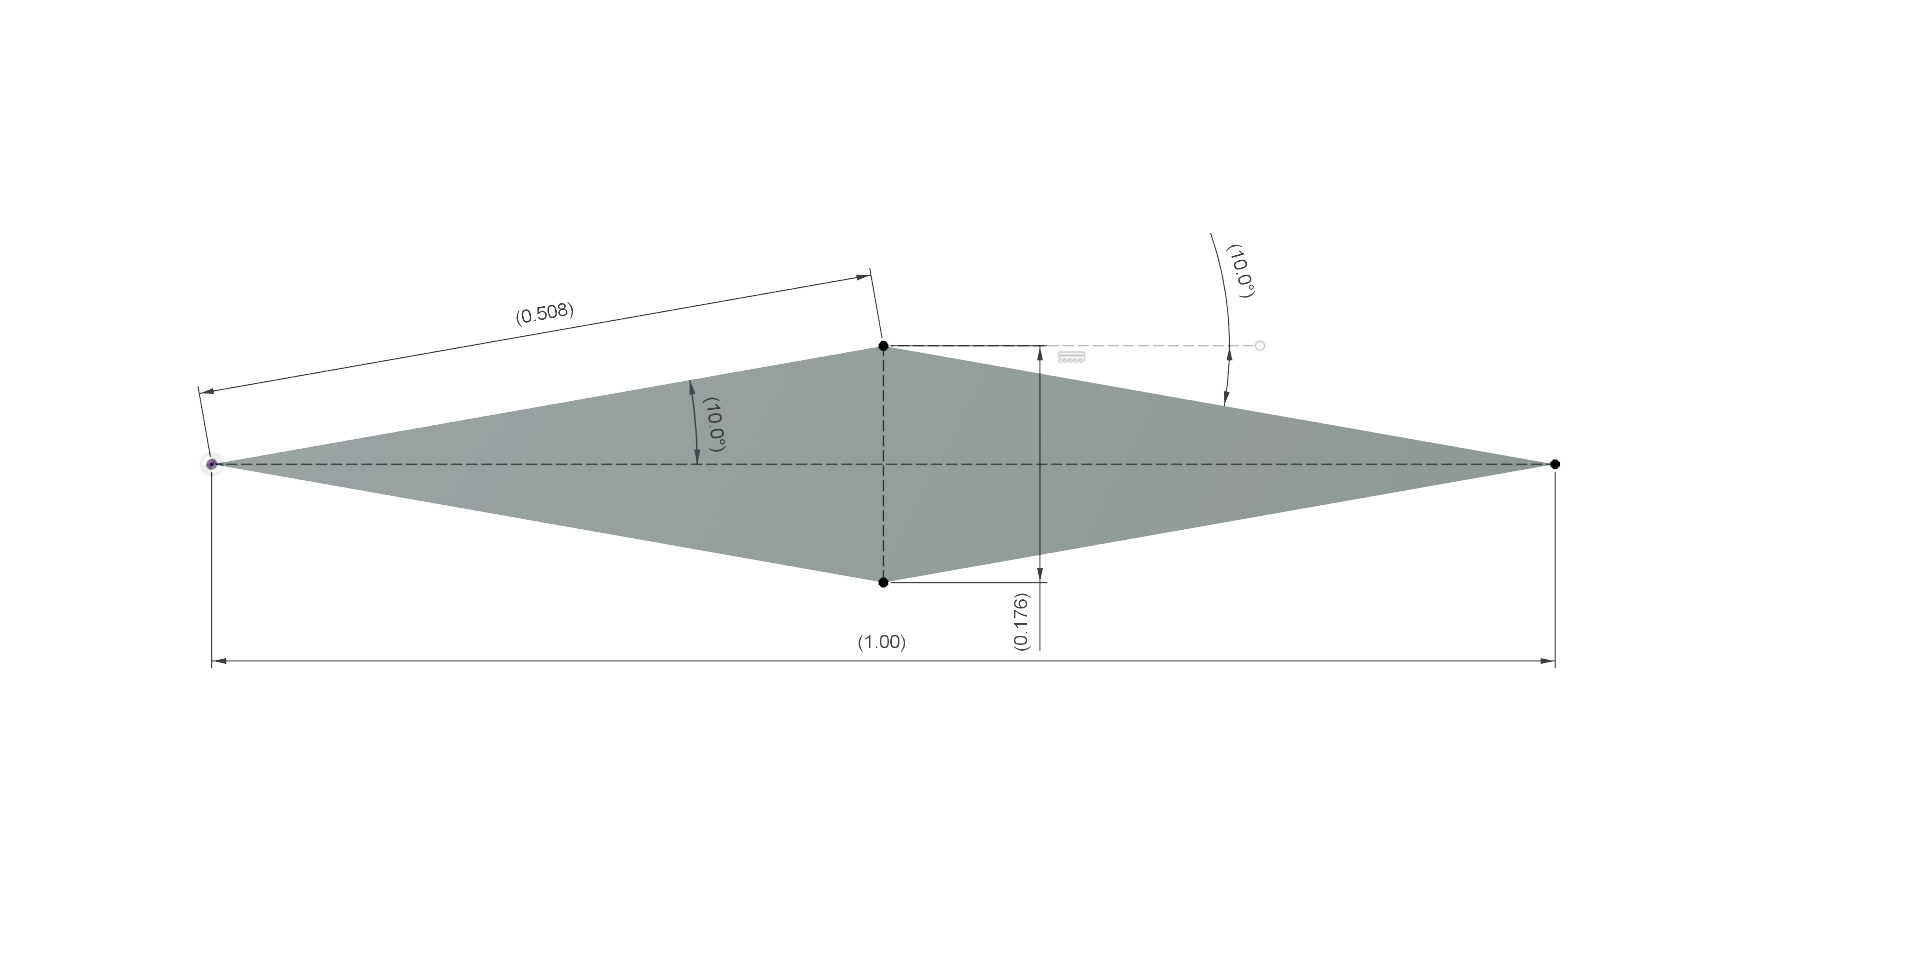
\includegraphics[width = \linewidth]{images/Diamond_Airfoil.png}
%       \caption{$\bR^{2}$}
%    \end{subfigure}   
%    \begin{subfigure}{0.495\linewidth}
%       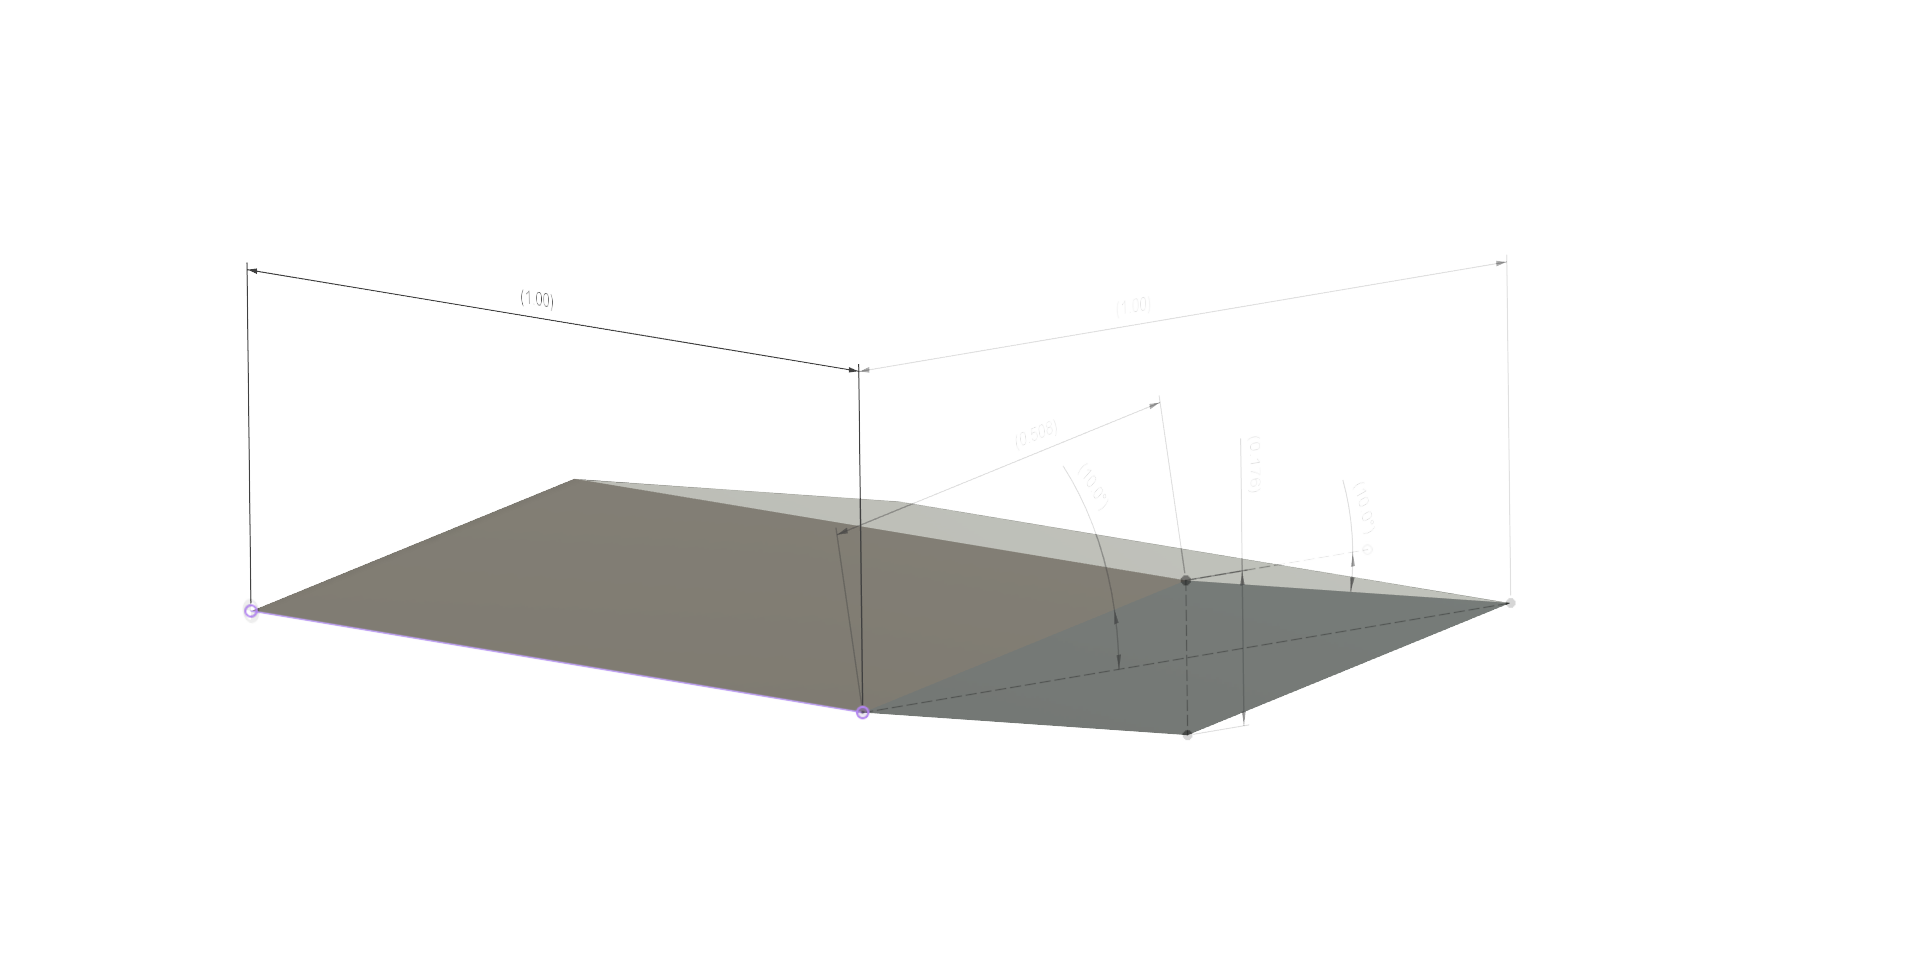
\includegraphics[width = \linewidth]{images/3D_Diamond_Section.png}
%       \caption{$\bR^{3}$}
%    \end{subfigure} 
% \end{figure}

% %-------------WILL CHANGE ONCE WE FINISH REPORT------------------------
% \section{Objectives}
% %-----------------------------------------------------------------
% \begin{enumerate}
%   \item \textbf{Establish the analytical reference solution for a $10^{\circ}$ half‑angle diamond at $M_{\infty}=3$.}\\[2pt]
%         \textit{Deliverables:} shock‑wave angle $\beta$ from the $\theta$–$\beta$–$M$ relation and the stagnation‑pressure ratio $p_{02}/p_{1}$ via normal‑shock\slash isentropic formulas.

%   \item \textbf{Quantify numerical error for the two‑dimensional Euler simulation.}\\[2pt]
%         \textit{Deliverables:} three successively refined meshes, Grid‑Convergence Index (GCI) for $\beta$ and $p_{0,\text{apex}}$, and a center‑line $C_{p}$ plot.

%   \item \textbf{Validate the converged 2‑D CFD solution against theory.}\\[2pt]
%         \textit{Success criterion:} \(\lvert \text{CFD} - \text{Theory} \rvert / \text{Theory} \le 2\%\) for both $\beta$ and $p_{0,\text{apex}}$.

%   \item \textbf{Assess three‑dimensional effects using a finite‑span diamond.}\\[2pt]
%         \textit{Deliverables:} span\slash chord specification, mesh/time refinement study, spanwise maps of $\beta$ and $p_{0}$, and GCI on mid‑span data.

%   \item \textbf{Compare 3‑D CFD to experimental measurements and discuss discrepancies.}\\[2pt]
%         \textit{Deliverables:} table of published Mach‑3 wedge/diamond data, overlay plot (Theory | 2‑D CFD | 3‑D CFD | Experiment), and discussion of viscous thickening, shock curvature, and edge effects.

% \end{enumerate}

%--------------------------------------------------------------------
\section{Governing Equations}
%--------------------------------------------------------------------
The flow is assumed to be inviscid, compressible, non–reacting and
calorically perfect (isothermal) with a constant specific–heat ratio
$\gamma = 1.4$.  Under these hypotheses, the governing equations reduce
to the \emph{compressible Euler equations} complemented by the ideal–gas
law.  For completeness we also list the oblique‑shock relations that
form the theoretical reference for the diamond airfoil.

%--------------------------------------------------------------------
\subsection{Three-dimensional Compressible Euler equations}
%--------------------------------------------------------------------
From the assumptions of Euler equations, e.g., no body forces and inviscid and isothermal flow, the simplified form of the \textit{Navier-Stokes Equations} in \(\mathbb{R}^{3}\) reads:

\begin{itemize}
  \item Continuity:
        \begin{equation}
          \frac{\partial \rho}{\partial t}
          + \rho\!\left(
              \frac{\partial u}{\partial x}
            + \frac{\partial v}{\partial y}
            + \frac{\partial w}{\partial z}
          \right) = 0.
        \end{equation}

  \item X‑Momentum:
        \begin{equation}
          \frac{\partial (\rho u)}{\partial t}
          + \rho\!\left(
              \frac{\partial u^{2}}{\partial x}
            + \frac{\partial u v}{\partial y}
            + \frac{\partial u w}{\partial z}
          \right) = -\frac{\partial p}{\partial x}.
        \end{equation}

  \item Y-Momentum:
        \begin{equation}
          \frac{\partial (\rho v)}{\partial t}
          + \rho\!\left(
              \frac{\partial v u}{\partial x}
            + \frac{\partial v^{2}}{\partial y}
            + \frac{\partial v w}{\partial z}
          \right) = -\frac{\partial p}{\partial y}.
        \end{equation}

  \item Z‑Momentum:
        \begin{equation}
          \frac{\partial (\rho w)}{\partial t}
          + \rho\!\left(
              \frac{\partial w u}{\partial x}
            + \frac{\partial w v}{\partial y}
            + \frac{\partial w^{2}}{\partial z}
          \right) = -\frac{\partial p}{\partial z}.
        \end{equation}

  \item Energy:
        \begin{equation}
          \frac{\partial E}{\partial t}
          + E\!\left(
              \frac{\partial u}{\partial x}
            + \frac{\partial v}{\partial y}
            + \frac{\partial w}{\partial z}
          \right) = -p\!\left(
              \frac{\partial u}{\partial x}
            + \frac{\partial v}{\partial y}
            + \frac{\partial w}{\partial z}
          \right),
        \end{equation}
\end{itemize}

Thus, the conservative state vector is

\[
  \mathbf{U} =
  \begin{bmatrix}
    \rho \\[2mm]
    \rho u \\[2mm]
    \rho v \\[2mm]
    \rho w \\[2mm]
    E
  \end{bmatrix},
\qquad
E = \rho\!\left(e + \tfrac12(u^{2}+v^{2}+w^{2})\right).
\]

%---------------------------------------------------------------
And the flux vectors, using \(\mathbf{F},\mathbf{G},\mathbf{H}\) to denote fluxes in the
\(x\), \(y\) and \(z\) directions, respectively, are

\[
  \mathbf{F}(\mathbf{U}) =
  \begin{bmatrix}
    \rho u \\[2mm]
    \rho u^{2} + p \\[2mm]
    \rho u v \\[2mm]
    \rho u w \\[2mm]
    (E + p)\,u
  \end{bmatrix}, \quad
  \mathbf{G}(\mathbf{U}) =
  \begin{bmatrix}
    \rho v \\[2mm]
    \rho v u \\[2mm]
    \rho v^{2} + p \\[2mm]
    \rho v w \\[2mm]
    (E + p)\,v
  \end{bmatrix}, \quad
  \mathbf{H}(\mathbf{U}) =
  \begin{bmatrix}
    \rho w \\[2mm]
    \rho w u \\[2mm]
    \rho w v \\[2mm]
    \rho w^{2} + p \\[2mm]
    (E + p)\,w
  \end{bmatrix}.
\]

With these definitions, the conservative form of Euler system in $\mathbb{R}^{3}$ reads

\begin{equation}
  \frac{\partial \mathbf{U}}{\partial t}
  + \frac{\partial \mathbf{F}}{\partial x}
  + \frac{\partial \mathbf{G}}{\partial y}
  + \frac{\partial \mathbf{H}}{\partial z} = \frac{\partial \mathbf{U}}{\partial t}
  + \nabla \cdot \mathbf{F}(\mathbf{U}) = \mathbf{0},
  \label{eq:euler3D}
\end{equation}
with state vector and flux tensor
\begin{align}
  \mathbf{U} &=
  \begin{bmatrix}
    \rho\\
    \rho u\\
    \rho v\\
    \rho w\\
    E
  \end{bmatrix}, &
  \mathbf{F}(\mathbf{U}) &=
  \begin{bmatrix}
    \rho \mathbf{u}\\[2pt]
    \rho \mathbf{u}\otimes\mathbf{u} + p\mathbf{I}\\[2pt]
    (E+p)\mathbf{u}
  \end{bmatrix},
\end{align}
where $\rho$ is the density, $\mathbf{u}=(u,v,w)^{\mathsf{T}}$ the
velocity, $E=\rho\bigl(e+\tfrac12\lVert\mathbf{u}\rVert^{2}\bigr)$ the total‐energy
per unit volume and $p$ the static pressure. This is the basis for the finite‑volume discretisation implemented in \textsc{OpenFOAM} for the 3‑D diamond‑airfoil simulations. Note: $\lVert\mathbf{u}\rVert \;=\; \sqrt{u^{2}+v^{2}+w^{2}}.$
\vspace{2.5mm}
In the quasi‑2‑D case ($w\!=\!0$) Eq.~\eqref{eq:euler3D} reduces to the familiar 2‑D expressions below:
\begin{equation}
   \frac{\partial \textbf{U}}{\partial t} + \frac{\partial \textbf{F}}{\partial x} + \frac{\partial \textbf{G}}{\partial y} = 0
\end{equation}

%--------------------------------------------------------------------
\subsection{Equation of state and thermodynamic closure}
%--------------------------------------------------------------------
The \textit{Ideal Gas Law} is our equation of state that relates the variables, $\rho$ which is our fluid density, $p$ the local pressure, $R$ the molecular gas constant, and $T$ the local temperature. 

\begin{equation}
   p = \rho RT 
   \label{IGL}
\end{equation}

Using the first law of Thermodynamics, $p$ can be related to the specific internal energy $e$ and the specific heat ratio $\gamma$ by:

\begin{equation}
   e = \frac{p}{\rho(\gamma-1)}
\end{equation}

These can be combined for a new expression that expresses \( p \) entirely in terms of the state vector \( \mathbf{U} \), allowing the flux vectors to be evaluated directly from conserved quantities. This closes the system.

\begin{equation}
    p = (\gamma - 1)\left(E - \frac{1}{2} \rho\lVert\mathbf{u}\rVert^{2}\right)
\end{equation}
%--------------------------------------------------------------------
\subsection{Local Sound Speed and Mach Number}
%--------------------------------------------------------------------
To analyze compressible flow behavior, we often need the local sound speed and Mach number.
The local speed of sound and Mach number follow directly:
\begin{itemize}
  \item Speed of sound, \( a \):
  \begin{equation}
    a = \sqrt{\gamma p/\rho}, \qquad
    \label{speedofsound}
  \end{equation}
  \item Mach number, \( M \) 
  \begin{equation}
    M = \frac{\lVert\mathbf{u}\rVert}{a}.
    \label{Mach_equation}
  \end{equation}
\end{itemize}

%--------------------------------------------------------------------
\subsection{Oblique‑shock theory ($\theta$–$\beta$–$M$ relation)}
%--------------------------------------------------------------------
For a sharp diamond airfoil the leading edges behave locally as two
identical wedges that deflect the flow by a half‑angle $\theta$.  The
shock‑wave angle $\beta$ is obtained from the classical $\theta$–$\beta$–$M$ equation
\begin{equation}
  \tan\theta \;=\;
  \frac{2\cot\beta\,(M_1^{2}\sin^{2}\beta-1)}
       {M_1^{2}(\gamma+\cos2\beta)+2},
  \label{eq:theta-beta-M}
\end{equation}
where $M_{1}$ is the upstream Mach number.  We always select the weak‑
shock root ($\beta < 90^{\circ}$).

Once $\beta$ is known the component of the Mach number normal to the shock can be calculated
\begin{equation}
  \boxed{\,M_{n1} = M_{1}\sin\beta\,}.
  \label{eq:Mn1}
\end{equation}
Equation~\eqref{eq:Mn1} acts as a bridge: it converts the
two‑dimensional oblique‑shock problem into an equivalent
one‑dimensional \emph{normal‑shock} problem, enabling the use of
standard jump and isentropic relations.

%---------------------------------------------------------------
\subsection{Normal‑Shock and Isentropic Relations (using $M_{n1}$)}
%---------------------------------------------------------------

\subsubsection*{Normal‑shock jumps}
\begin{align}
  \frac{p_{2}}{p_{1}}
    &= 1 + \frac{2\gamma}{\gamma+1}\bigl(M_{n1}^{2}-1\bigr),
    \label{eq:p2p1}\\[4pt]
  \frac{\rho_{2}}{\rho_{1}}
    &= \frac{(\gamma+1)M_{n1}^{2}}
            {(\gamma-1)M_{n1}^{2}+2},
    \label{eq:rho2rho1}\\[4pt]
  M_{n2}^{2}
    &= \frac{1+\tfrac12(\gamma-1)M_{n1}^{2}}
            {\gamma M_{n1}^{2}-\tfrac12(\gamma-1)}.
    \label{eq:Mn2}
\end{align}

\subsubsection*{Total‑pressure ratio across the shock}
\begin{equation}
  \frac{p_{02}}{p_{01}} =
    \left[\frac{(\gamma+1)M_{n1}^{2}}
               {(\gamma-1)M_{n1}^{2}+2}\right]^{\gamma/(\gamma-1)}
    \left[\frac{\gamma+1}
               {2\gamma M_{n1}^{2}-(\gamma-1)}\right]^{1/(\gamma-1)}.
  \label{eq:total-pressure-ratio}
\end{equation}

\subsubsection*{Isentropic relations (regions 1 and 2)}
\begin{equation}
  \frac{p_{01}}{p_{1}}
    = \left[1+\frac{\gamma-1}{2}M_{1}^{2}\right]^{\gamma/(\gamma-1)},
  \qquad
  \frac{p_{02}}{p_{2}}
    = \left[1+\frac{\gamma-1}{2}M_{2}^{2}\right]^{\gamma/(\gamma-1)},
  \label{eq:isentropic}
\end{equation}
with
\begin{equation}
  M_{2} = \frac{M_{n2}}{\sin(\beta-\theta)}.
  \label{eq:M2}
\end{equation}

\subsubsection*{Stagnation pressure at the apex}
\begin{equation}
  p_{\text{stag}}
  = p_{02}
  = \frac{p_{02}}{p_{01}}\,
    \frac{p_{01}}{p_{1}}\,
    p_{1},
  \label{eq:pstag}
\end{equation}
where the two ratios on the right‑hand side are given by
Eqs.~\eqref{eq:total-pressure-ratio} and~\eqref{eq:isentropic},
respectively.

%--------------------------CHANGE WHEN WE HAVE P VALUE----
\subsection{Reference stagnation pressure for the baseline case}
%--------------------------------------------------------------------
For the baseline configuration ($M_{\infty}=3$, $\theta = 10^{\circ}$),
Eqs.~\eqref{eq:theta-beta-M}–\eqref{eq:total-pressure-ratio} give
\[
  \beta = 27.38^{\circ}, 
  \quad
  M_{n1}=1.38,
  \quad
  \frac{p_{02}}{p_{01}} = 0.96.
\]
This value serves as the \emph{theoretical target} against which the
grid‑refined 2‑D CFD solutions will be validated before the
three‑dimensional extension.

% %-----------PLACEHOLDER, MOVE TO CONCLUSION----------------------------
% \subsection*{Summary}
% %--------------------------------------------------------------------
% Equations~\eqref{eq:euler3D}–\eqref{eq:total-pressure-ratio} fully define
% the inviscid compressible flow field and the analytical reference
% solution required for the objectives.  They form the
% foundation for both the OpenFOAM numerical model and the subsequent
% error analysis against oblique‑shock theory.

\section{Mesh Setup}
The mesh of the diamond-shaped wing is generated from \textit{OpenFOAM's} \texttt{blockMeshDict} which is set up as follows:
\subsection{2D}
In $\bR^{2}$:
\begin{figure}[H]
   \centering
   \begin{subfigure}{0.495\linewidth}
      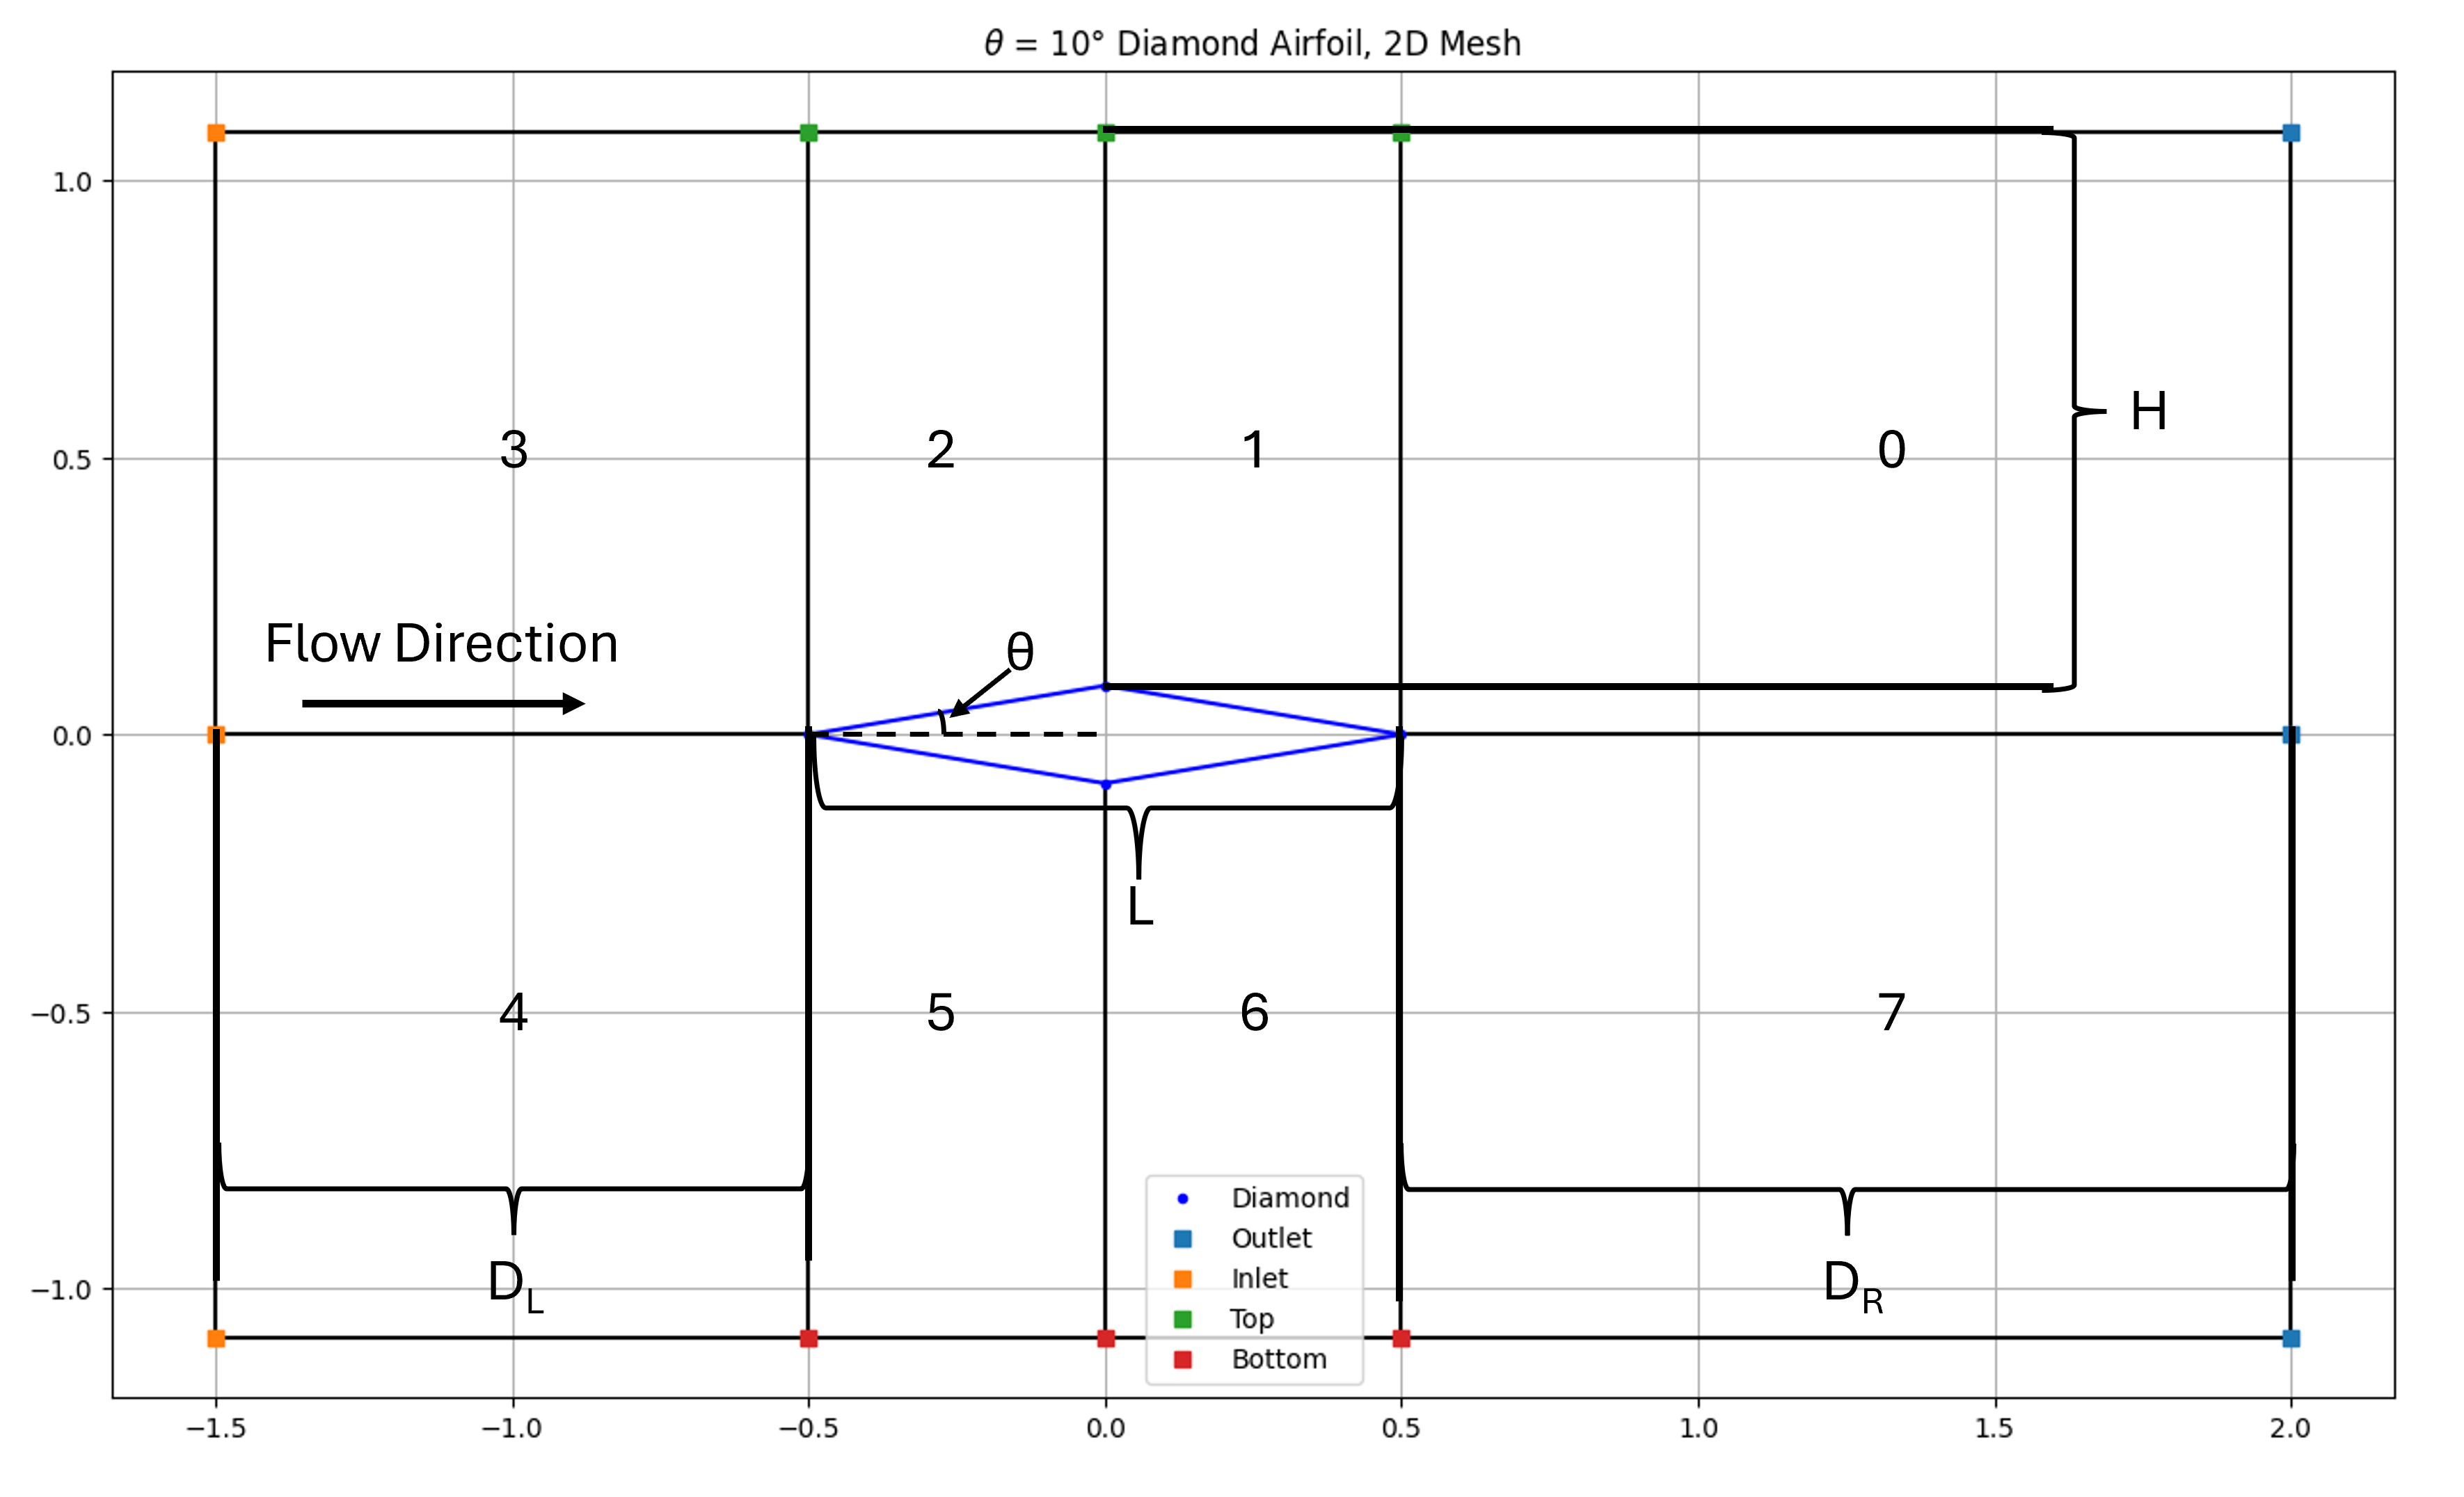
\includegraphics[width = \linewidth]{images/2D_Diamond_Airfoil_Mesh.png}
      \caption{2D Mesh Schematic}
   \end{subfigure}   
   \begin{subfigure}{0.475\linewidth}
      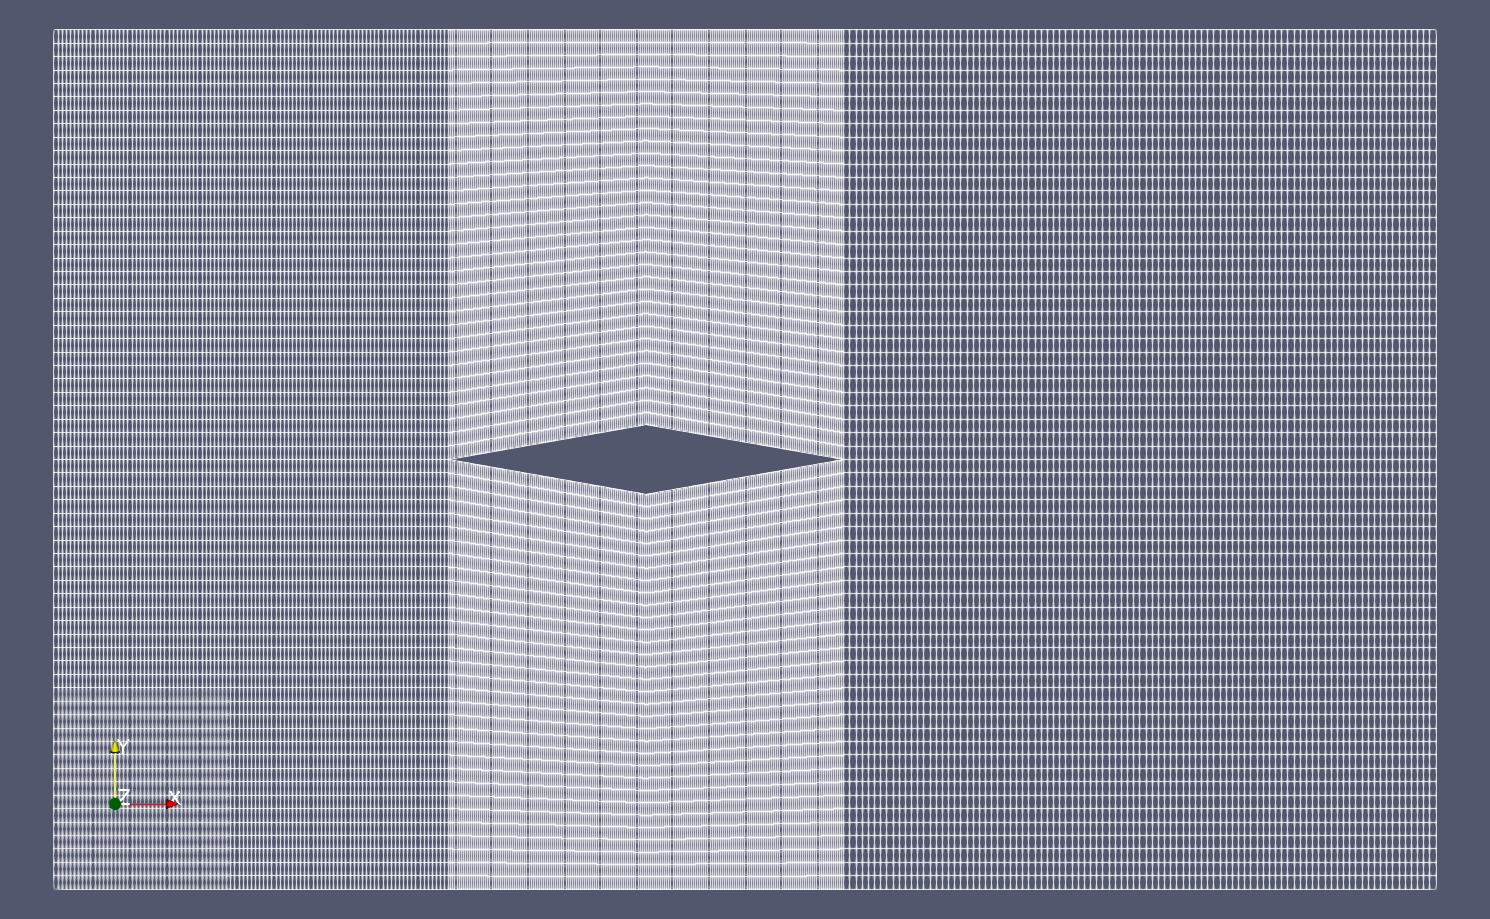
\includegraphics[width = \linewidth]{images/2D_Diamond_Airfoil_Mesh_PARAVIEW.png}
      \caption{2D Mesh in \textit{Paraview}}
   \end{subfigure} 
\end{figure}

Where for our case:
\begin{itemize}
   \item $L = 1.0$ (Chord)
   \vspace{2mm}
   \item $\theta = 10\degree$ (Deflection Angle)
   \vspace{2mm}
   \item $D_{L} = 1.0$ (Distance Left of the Diamond - Fore)
   \vspace{2mm}
   \item $D_{R} = 1.5$ (Distance Right of the Diamond - Aft)
   \vspace{2mm}
   \item $H = 1.0$ (Distance Above/Below the top/bottom-most point of the Diamond)
\end{itemize}

The size of the computational domain is then $(D_{L} + L + D_{R}) \times (2H + L\tan{(\theta)}) \times 0.1$. The \texttt{blockMeshDict} for the $\bR^{2}$ case can be found in the \hyperlink{code}{\textbf{Appendix}}.
\vspace{2.5mm}

\subsection{3D}
\begin{figure}[H]
  \centering
  
\begin{figure}[H]
   \centering
   \begin{subfigure}{0.55\linewidth}
      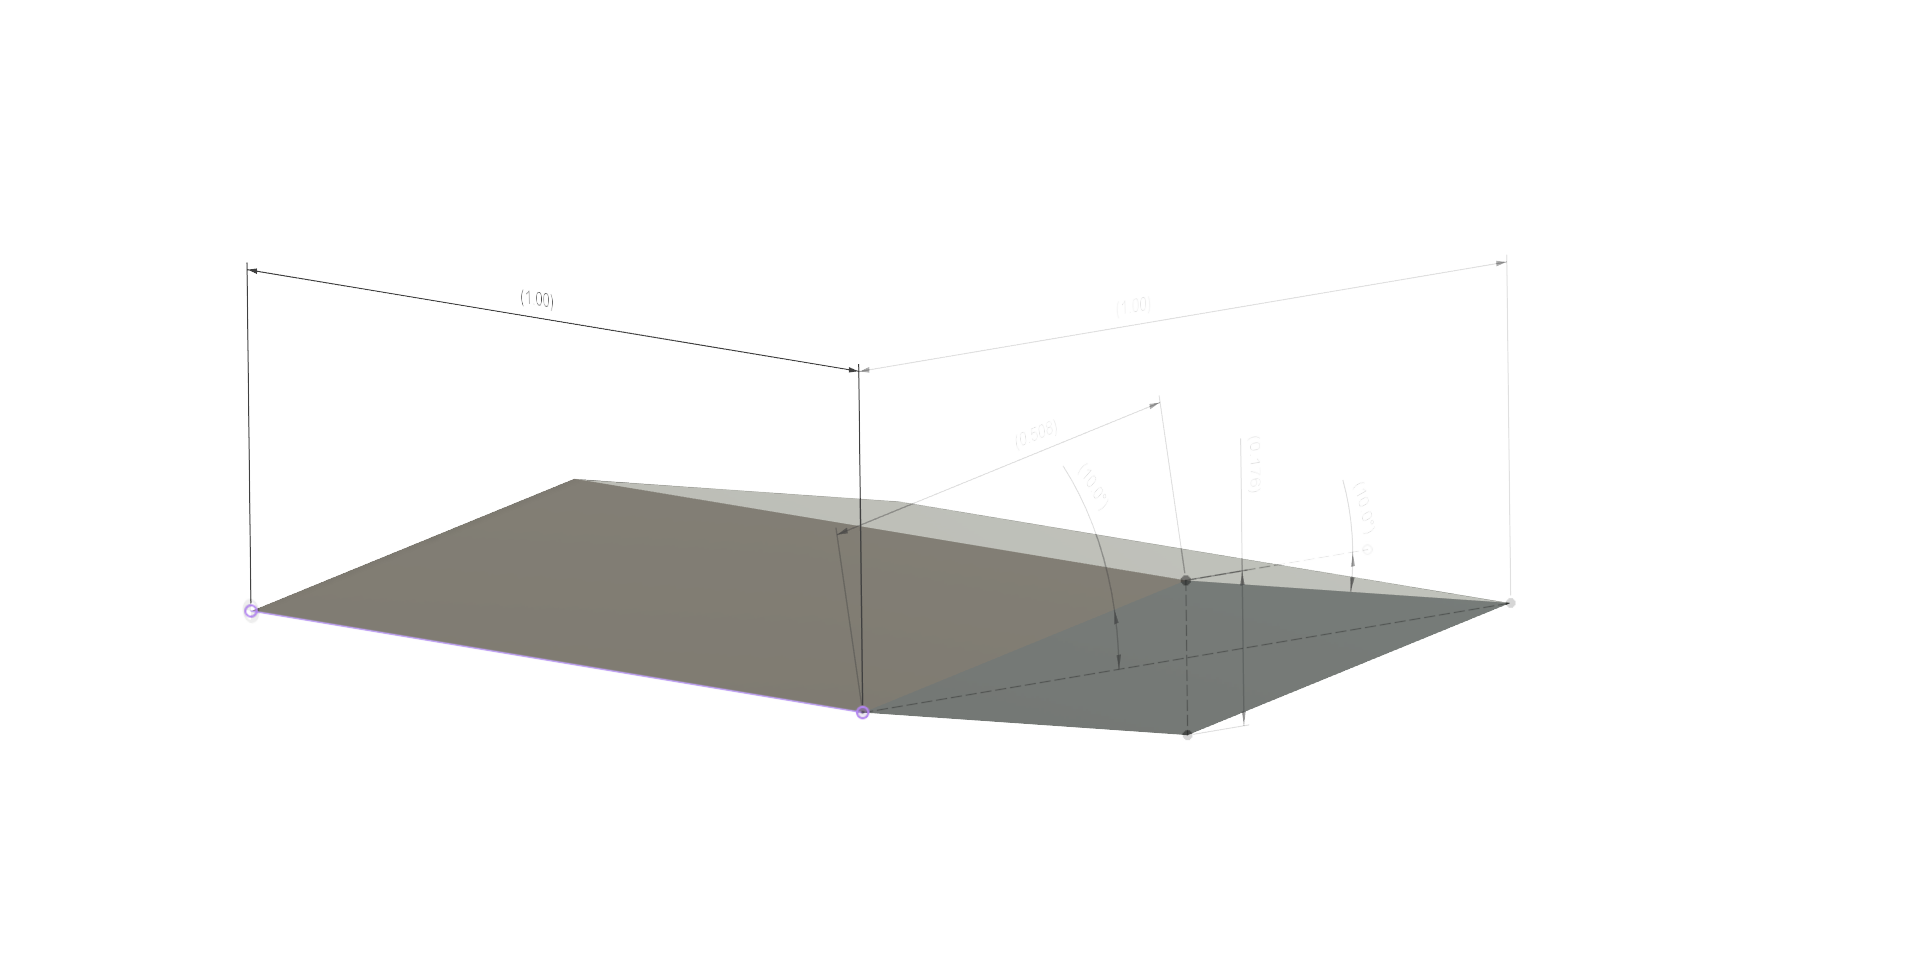
\includegraphics[width = \linewidth]{images/3D_Diamond_Section.png}
      \caption{CAD of Diamond Wing}
   \end{subfigure}   
   \begin{subfigure}{0.435\linewidth}
      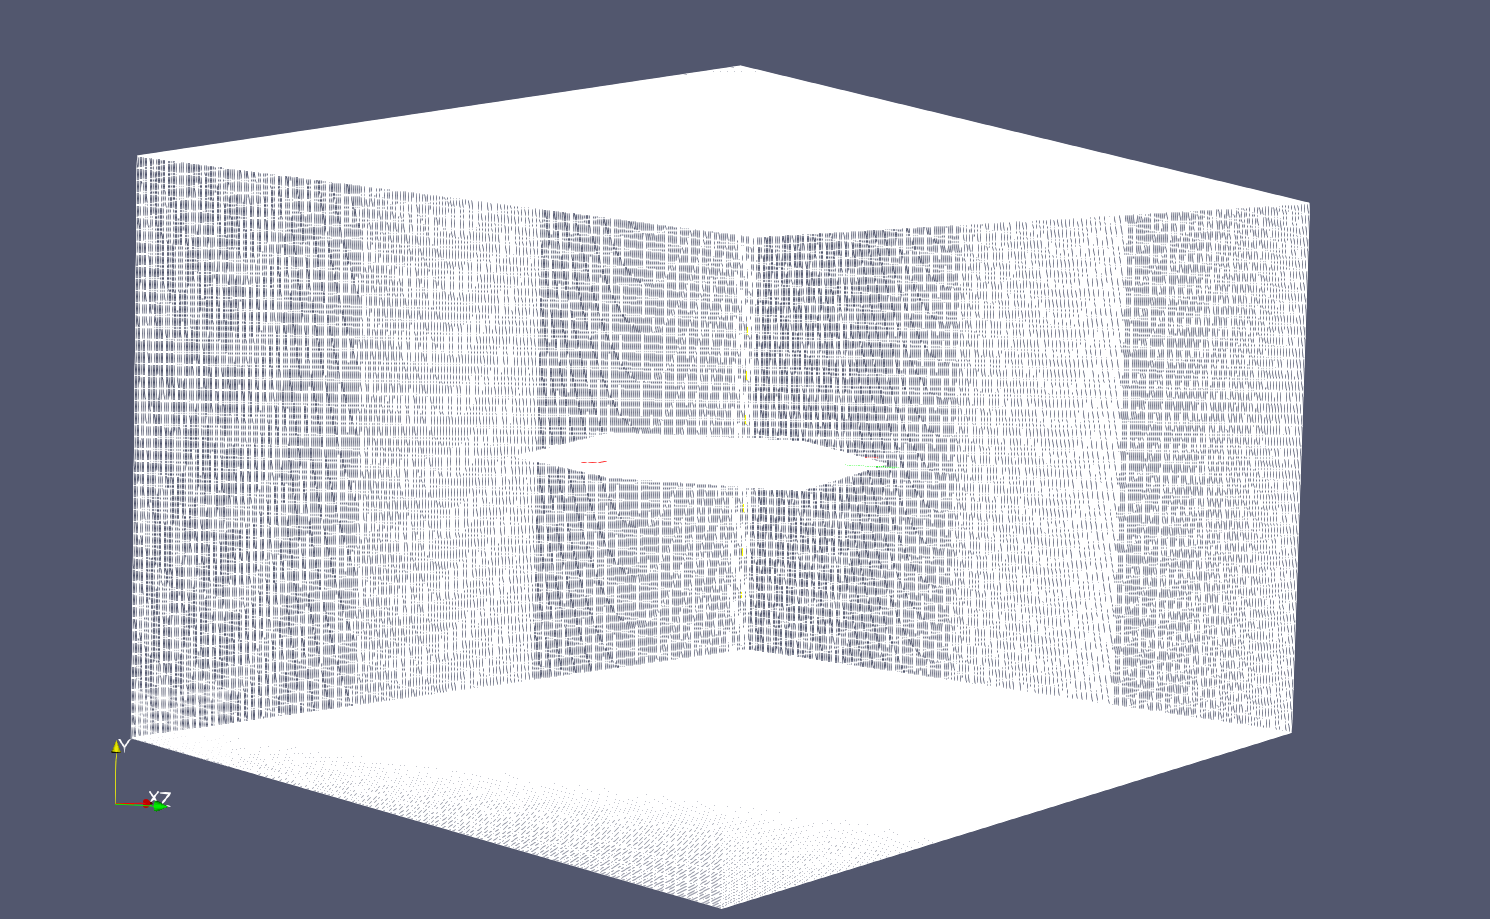
\includegraphics[width = \linewidth]{images/3D_Diamond_Mesh_PARAVIEW.png}
      \caption{3D Mesh in \textit{Paraview}}
   \end{subfigure} 
\end{figure}


\end{figure}

We introduce a new term $D_{Z} = 1.0$ which is the extension of the computational domain from diamond wing in the z-direction. We also add two new boundaries for the front and back walls as \texttt{symmetryPlane}'s to close the 3D domain. The span of our diamond is  $b = 1$. The \texttt{blockMeshDict} for the $\bR^{3}$ case can be found in the \hyperlink{code}{\textbf{Appendix}}. This \texttt{blockMeshDict} creates the bounding domain while Diamond-Shaped wing is made using CAD and the STL is meshed within the bounds using \texttt{snappyHexMesh}.
\vspace{2.5mm}

\section{Mesh Refinement and Comparison to OST}
In this section, we analyze three mesh resolutions: coarse, intermediate, and refined.
\begin{table}[H]
  \centering
  \begin{tabular}{|l|c|c|}
  \hline
  \textbf{MeshID} & \textbf{Cells} & $\Delta t$ [s]\\\hline
  Coarse  & 16,896  & 0.004\\  
  Intermediate  & 67,584  & 0.002\\
  Refined  & 1,081,344  & 0.0005\\\hline
  \end{tabular}
  \caption{\centering Mesh and Solver Parameters\\[2mm]}
  \label{tab:meshes}
  \end{table}
  
\subsection{First Coarse Solution}
For our coarse solution, we will visualize the properties pressure $p$, density $\rho$, velocity $\textbf{U}$, and temperature $T$ after simulating Mach 3 flow over the step for $T=4\; \text{s}$. 

\begin{figure}[H]
    \centering
    \begin{subfigure}{0.495\linewidth}
        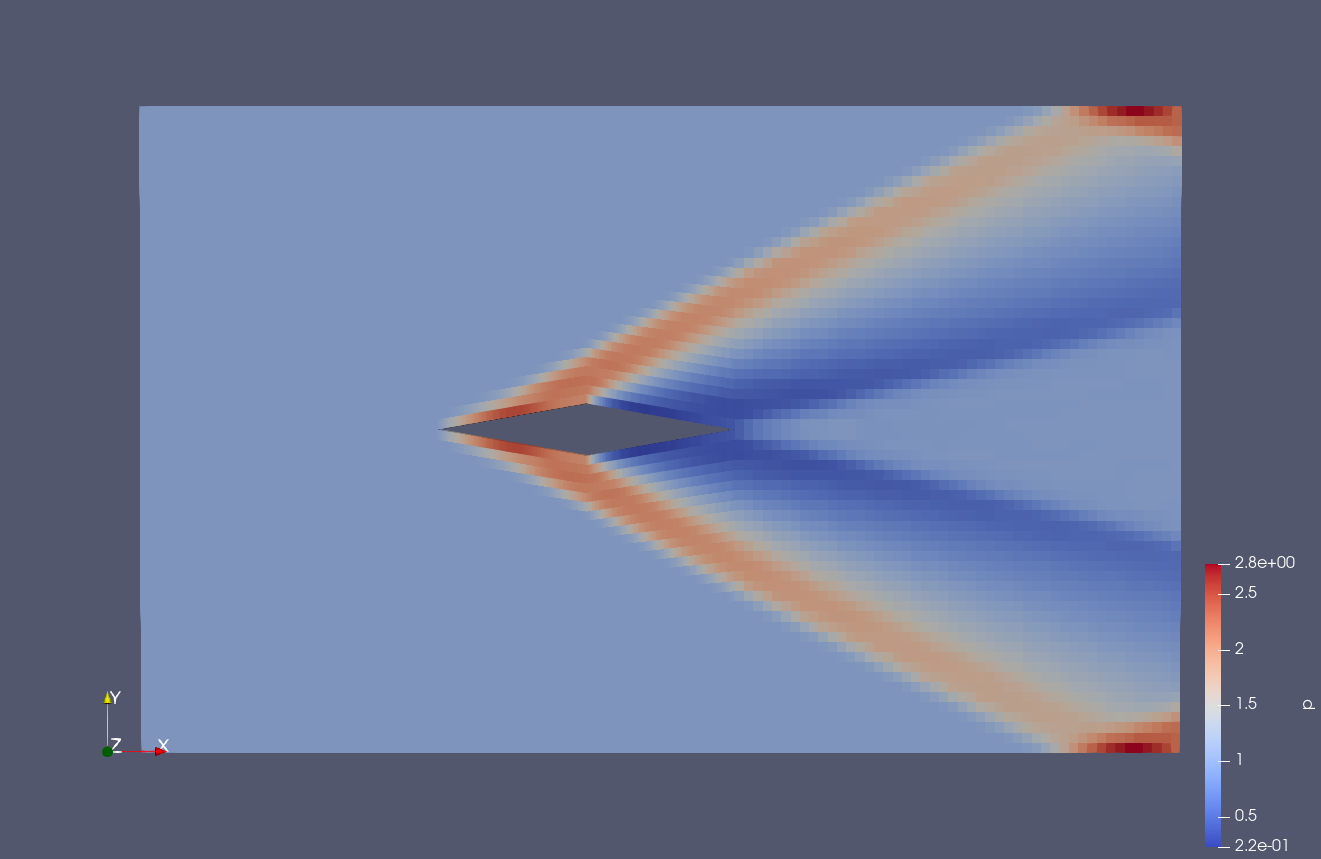
\includegraphics[width = \linewidth]{images/2D-coarse-pressure.png}
        \caption{Pressure $p$}
    \end{subfigure}
    \begin{subfigure}{0.495\linewidth}
        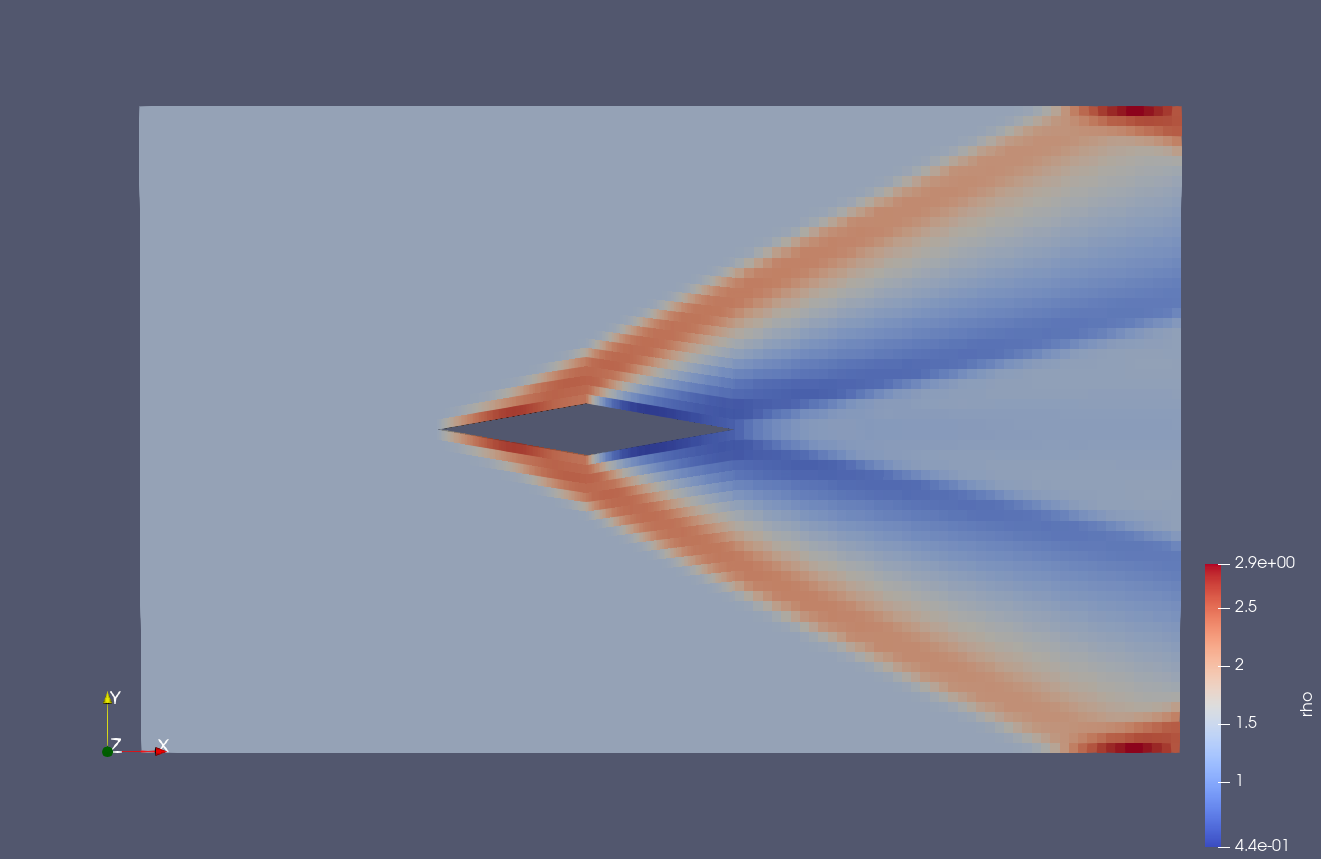
\includegraphics[width = \linewidth]{images/2D-coarse-rho.png}
        \caption{Density $\rho$}
    \end{subfigure}
    \vspace{1.5mm}

    \begin{subfigure}{0.495\linewidth}
        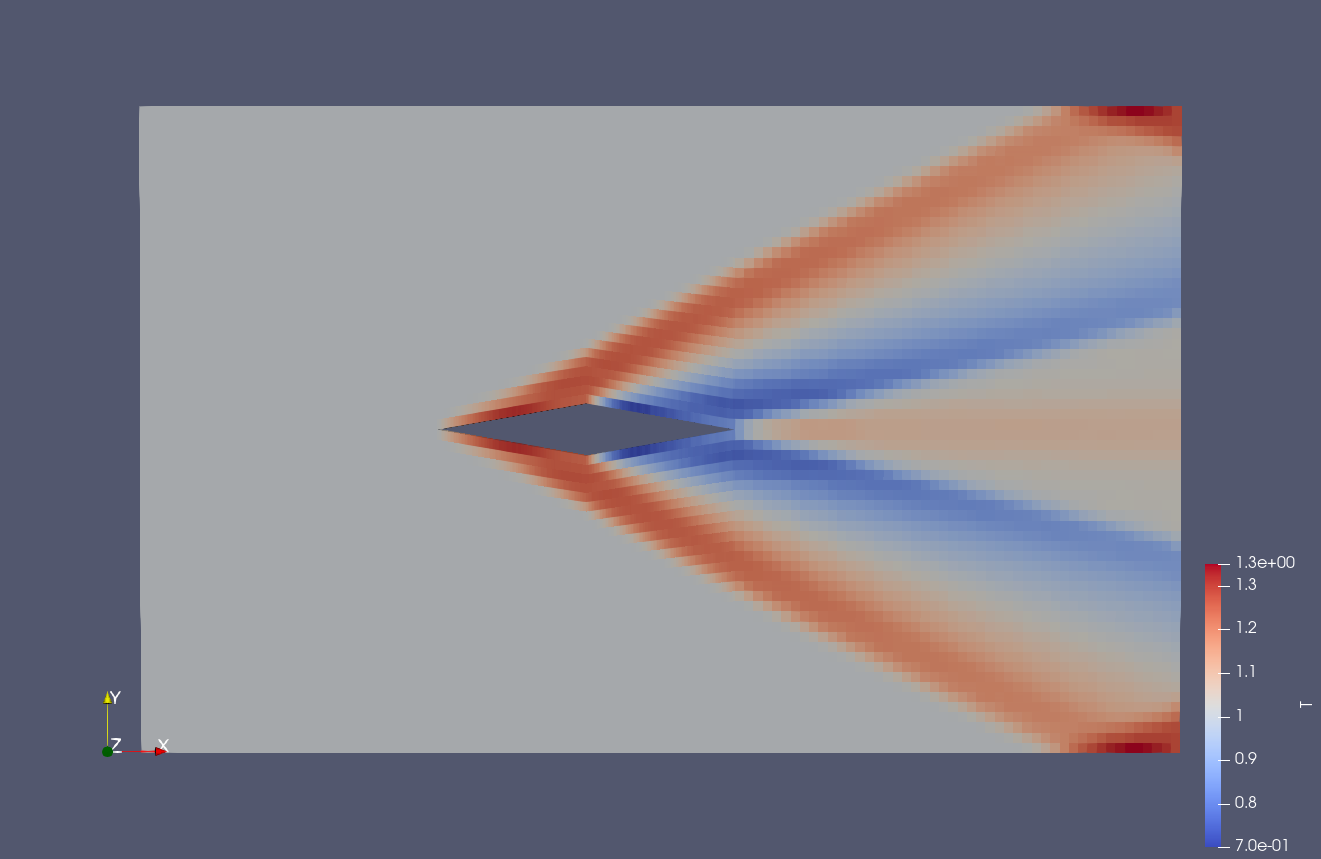
\includegraphics[width = \linewidth]{images/2D-coarse-temp.png}
        \caption{Temperature $T$}
    \end{subfigure}
    \begin{subfigure}{0.495\linewidth}
        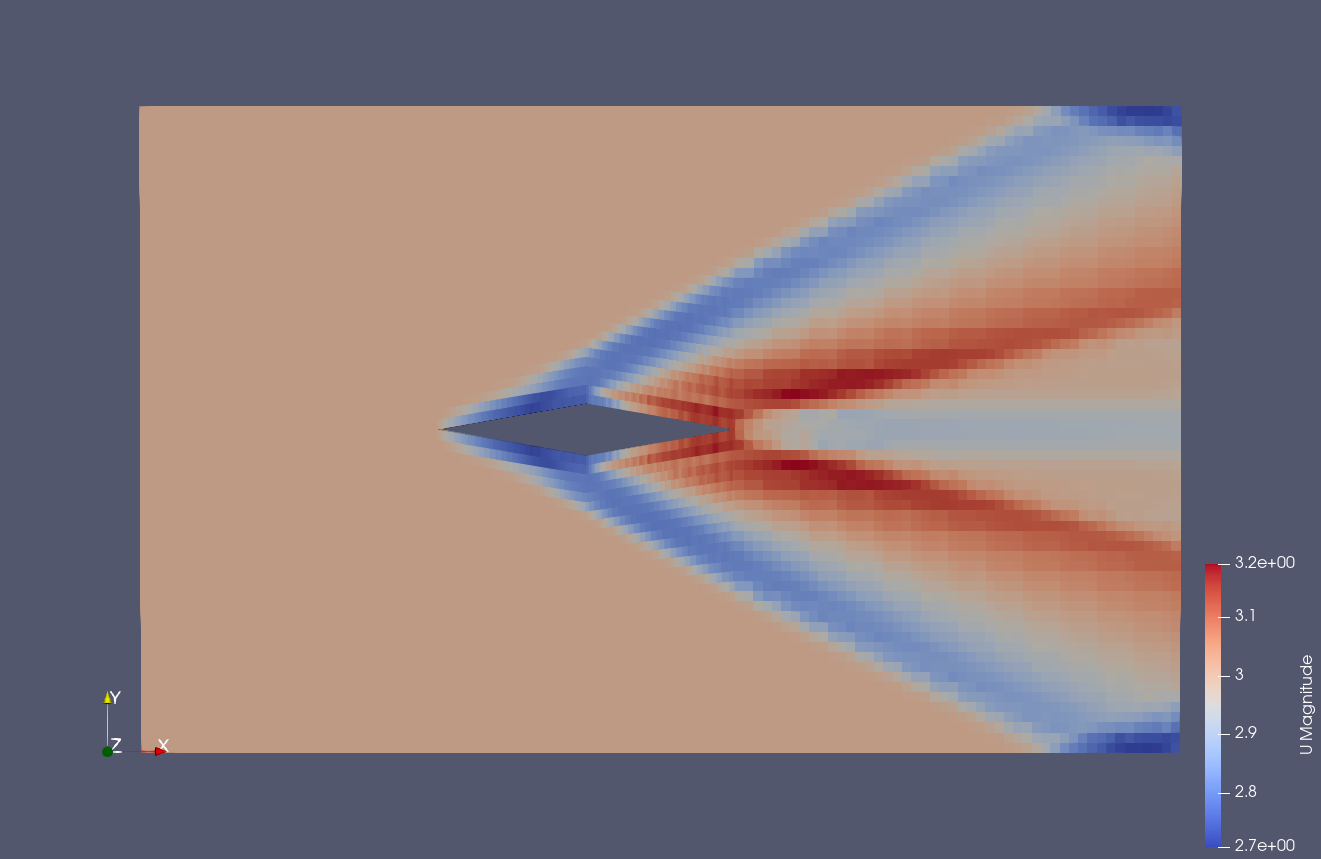
\includegraphics[width = \linewidth]{images/2D-coarse-velocity.png}
        \caption{Magnitude of Velocity $|\textbf{U}|$}
    \end{subfigure}
    \vspace{1.5mm}
    \caption{Properties of Coarse Mesh Solution}
    \label{coarsesolution}
\end{figure}
\vspace{1mm}

Using the built-in calculator in \textit{Paraview}, we are able to employ Equations \ref{speedofsound} and \ref{Mach_equation} to visualize the Mach and Speed of Sound in our supersonic simulation.

\begin{figure}[H]
    \centering
    \begin{subfigure}{0.495\linewidth}
        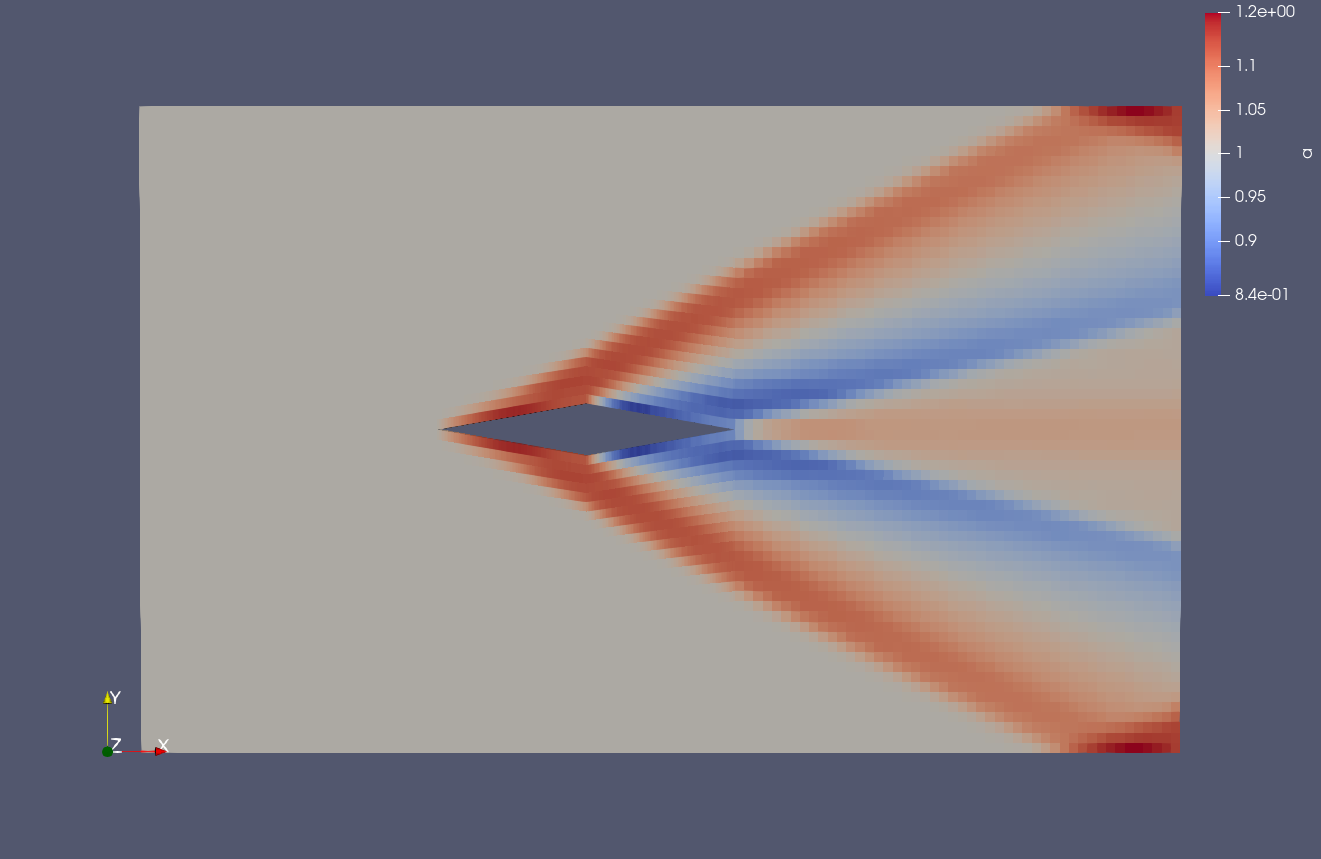
\includegraphics[width = \linewidth]{images/2D-coarse-a.png}
        \caption{Speed of Sound $a$}
    \end{subfigure}    
    \begin{subfigure}{0.495\linewidth}
        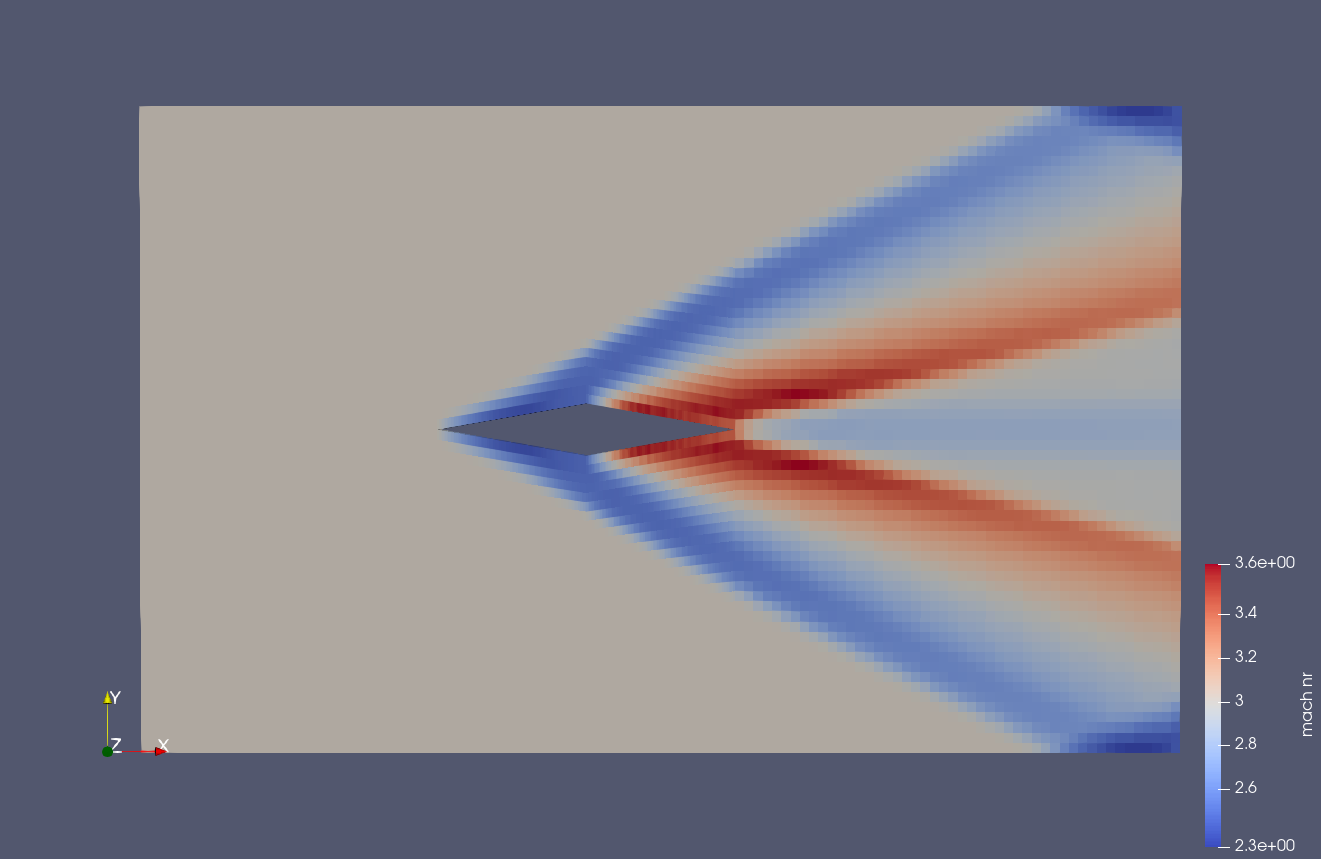
\includegraphics[width = \linewidth]{images/2D-coarse-machnr.png}
        \caption{Mach No. $M$}
    \end{subfigure}    
    \caption{Mach and Speed of Sound of Coarse Mesh Solution}
    \label{machandsoundspeed}
\end{figure}

\subsection{Intermediate and Refined Solution}
\begin{figure}[H]
  \centering
  \begin{subfigure}{0.495\linewidth}
      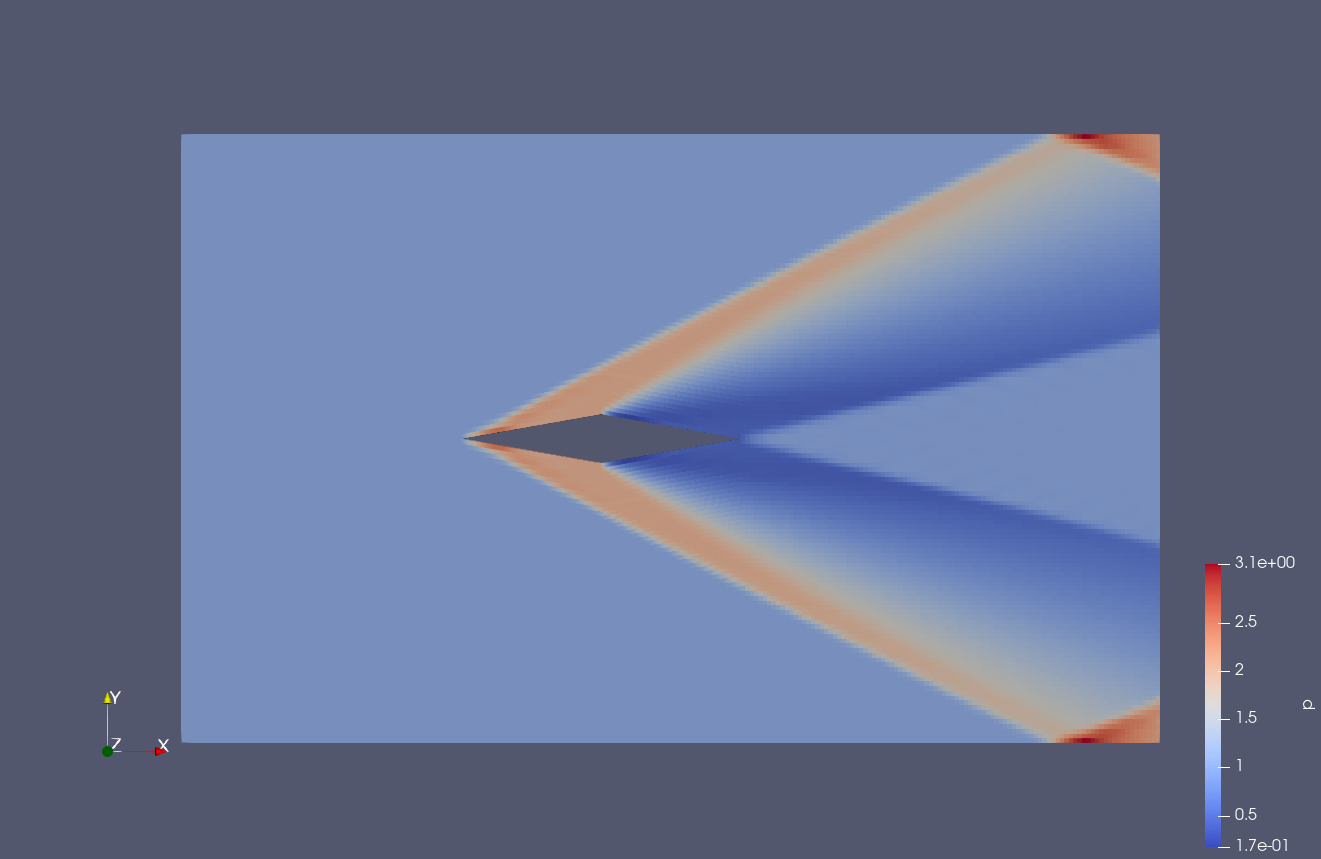
\includegraphics[width = \linewidth]{images/2D-interm-pressure.png}
      \caption{Intermediate Mesh Solution, Pressure $p$}
  \end{subfigure}
  \begin{subfigure}{0.495\linewidth}
      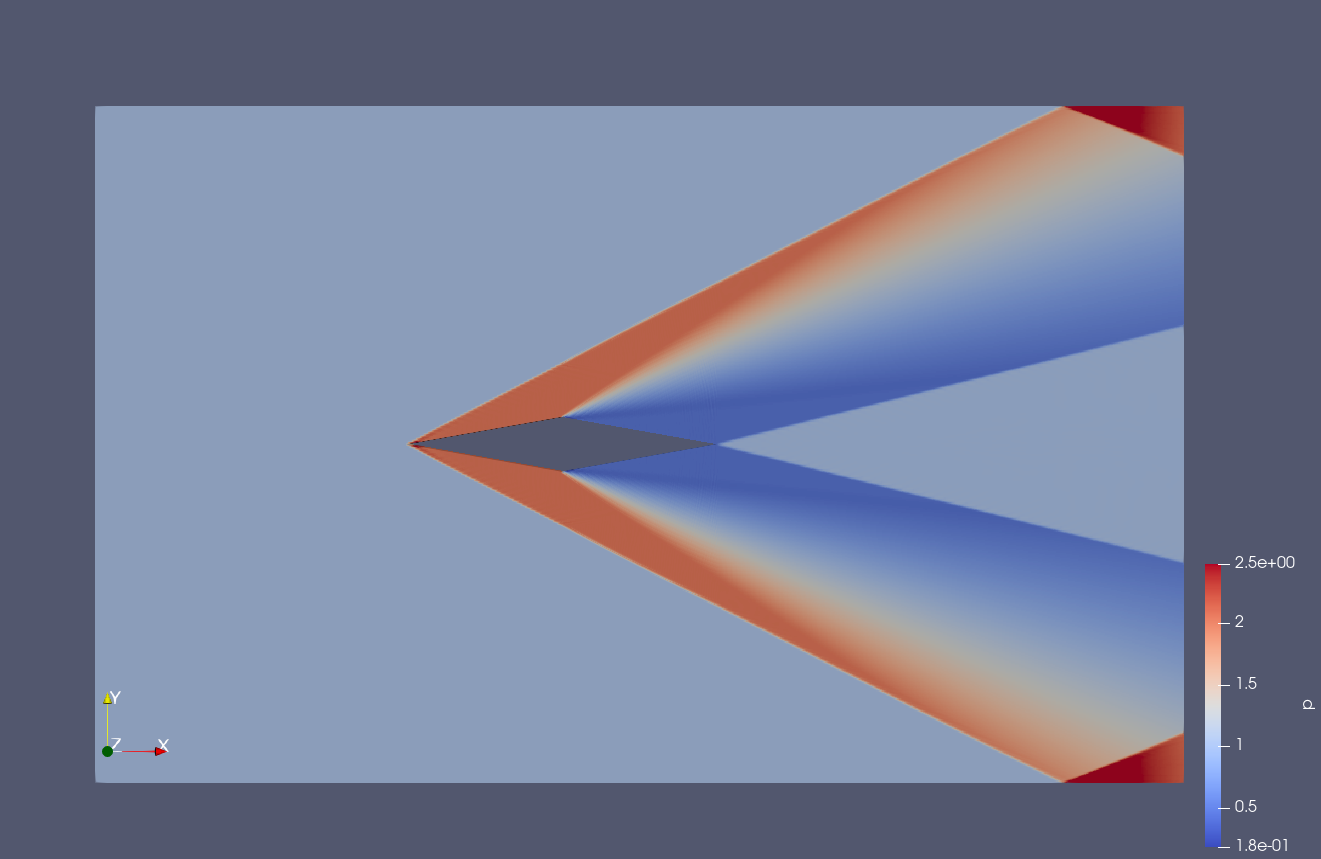
\includegraphics[width = \linewidth]{images/2D-refine-pressure.png}
      \caption{Refined Mesh Solution, Pressure $p$}
  \end{subfigure}
  \vspace{2.5mm}
\end{figure}

\subsection{Wave Angle and Pressure}
Pressure along the forward facing top surface for all resolutions is shown in the Figures below.
\begin{figure}[H]
  \centering
  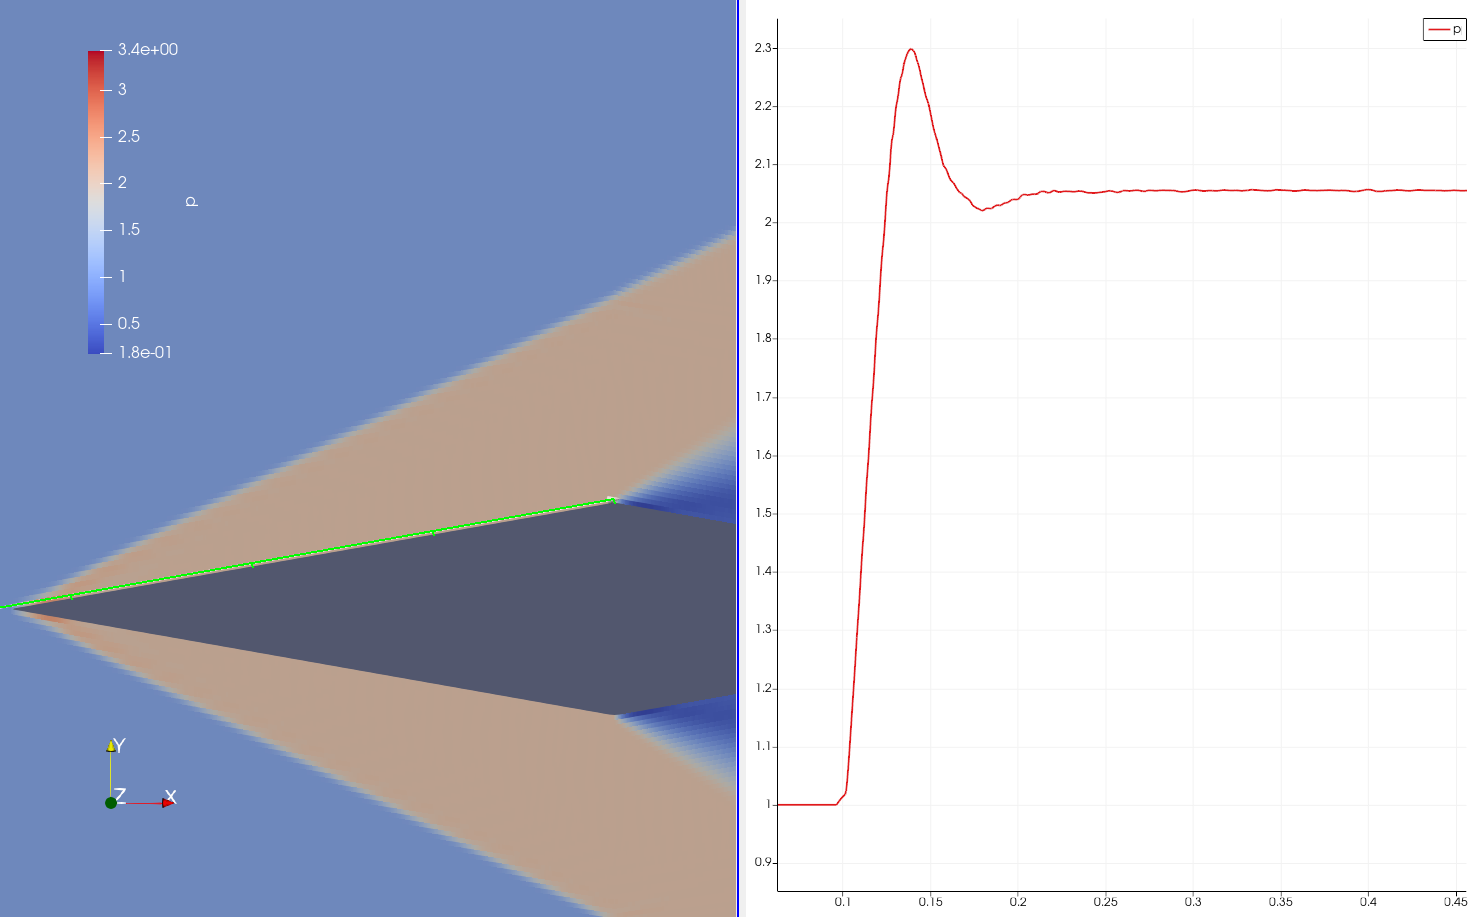
\includegraphics[width = 0.75\linewidth]{images/Pressure_NX8_Plot.png}
  \caption{Pressure captured along the top front surface of the diamond wing section}
\end{figure}

To calculate wave angle, we place a vertical line at a distance \(x=L/2\) downstream of the wedge apex (nose) and measure the shock height above the surface as \(y\).  Denoting by \(\beta\) the angle between the shock and the wedge surface, simple trigonometry gives
\begin{figure}[H]
  \centering
  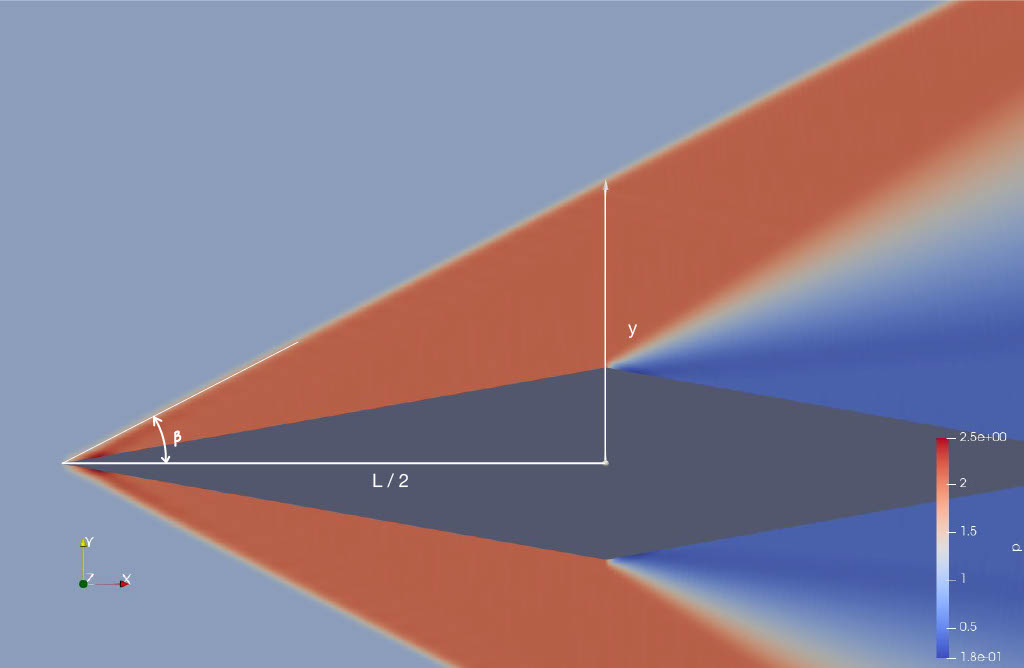
\includegraphics[width=0.6\textwidth]{images/angle-visual.jpg} 
  \caption{Calculation of Shock Angle Visual} 
  \label{fig:your-label}
\end{figure}


\[
  \beta 
  = \arctan\!\biggl(\frac{y}{L/2}\biggr)
  = \arctan\!\Bigl(\tfrac{2y}{L}\Bigr).
\]
The oblique‐shock angle \(\beta\) is measured with respect to the incoming flow direction, and the wedge deflection angle is
\(\theta=10^\circ\).  From the geometry (see Fig. 7),
\[
  \beta \;=\;\frac{y}{L/2}
  \;=\;\frac{2\,y}{L}
\]

\begin{table} [H]
  \centering
  \caption{Computed shock‐wave angle $\beta$ for different solution levels}
  \label{tab:shock_angles}
  \begin{tabular}{lccc}
    \toprule
    \textbf{MeshID} & {$y$ (m)} & {$L$ (m)} & {$\beta$ ($^{\circ}$)} \\
    \midrule
    Coarse         & 0.256   & 0.10   & 27.11 \\
    Intermediate   & 0.258   & 0.10   & 27.29 \\
    Refined        & 0.260   & 0.10   & 27.47 \\
    Theory         &         &        & 27.38 \\
    \bottomrule
  \end{tabular}
\end{table}
\noindent Table~\ref{tab:shock_angles} compares the computed shock angles for three mesh resolutions against the theoretical value $\beta_{\rm theory}=27.38^\circ$.  We define
\[
\Delta\beta = \beta_{\rm comp}-\beta_{\rm theory},
\qquad
\varepsilon = \frac{|\Delta\beta|}{\beta_{\rm theory}}\times100\%.
\]
The coarse mesh underestimates the angle by $\Delta\beta=-0.27^\circ$ ($\varepsilon=1.0\%$), while the intermediate mesh gives $\Delta\beta=-0.09^\circ$ ($\varepsilon=0.33\%$) and the refined mesh $\Delta\beta=+0.09^\circ$ ($\varepsilon=0.33\%$).  Errors fall below $0.1^\circ$ on the finer grids, indicating convergence toward the theoretical solution.  


\section{In Three Dimensions}
\begin{figure}[H]
  \centering
  \begin{subfigure}{0.495\linewidth}
     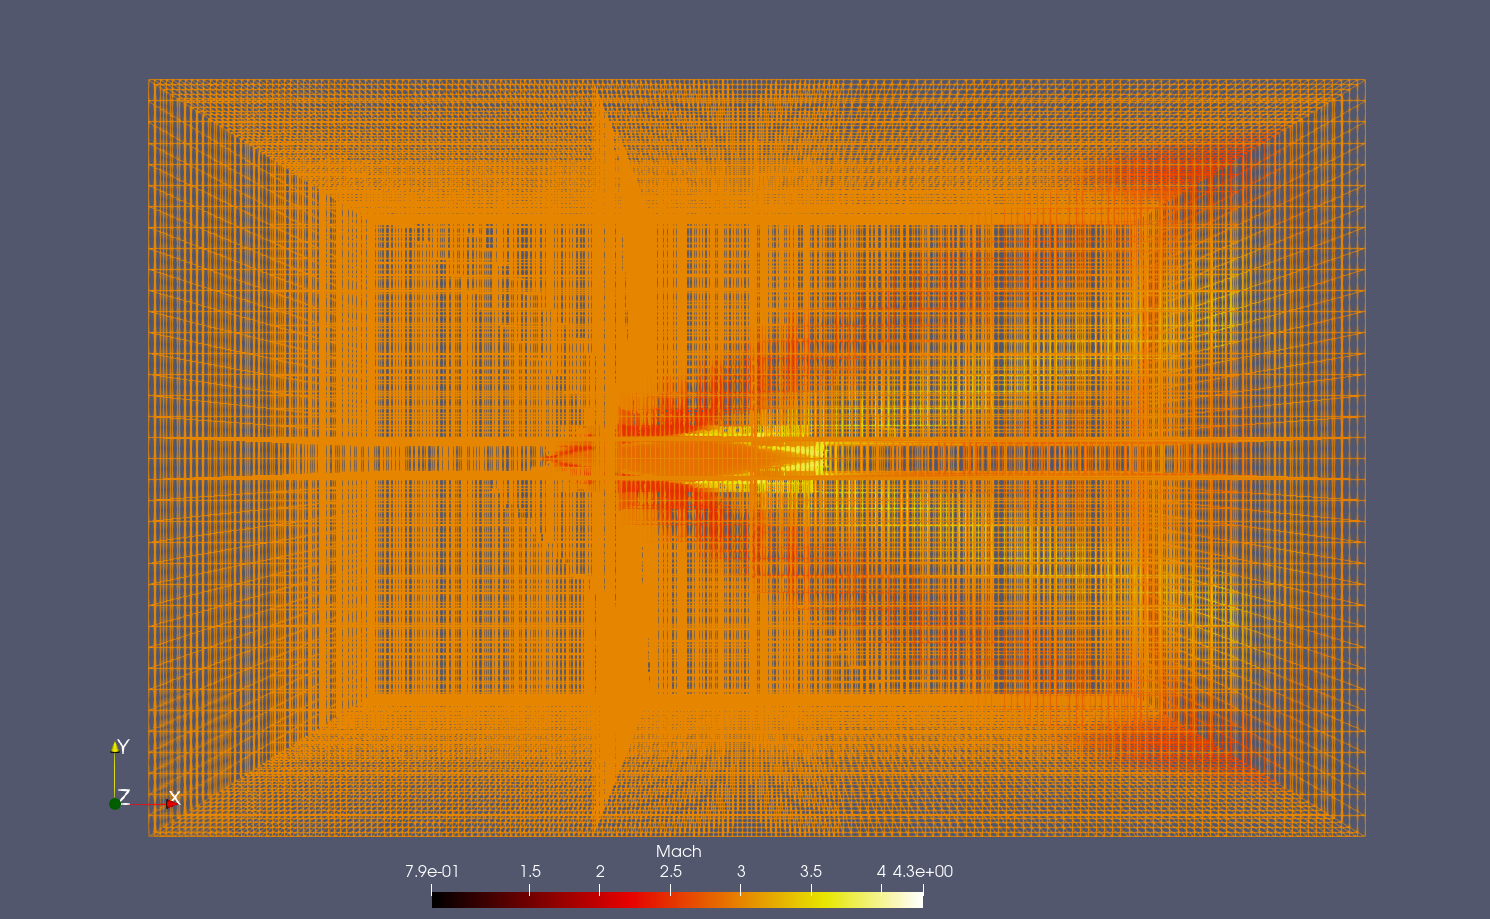
\includegraphics[width = \linewidth]{images/3D_Diamond_Wireframe_Coarse_Mach_PARAVIEW.png}
     \caption{3D Mesh in Wireframe view}
  \end{subfigure} 
  \begin{subfigure}{0.4\linewidth}
    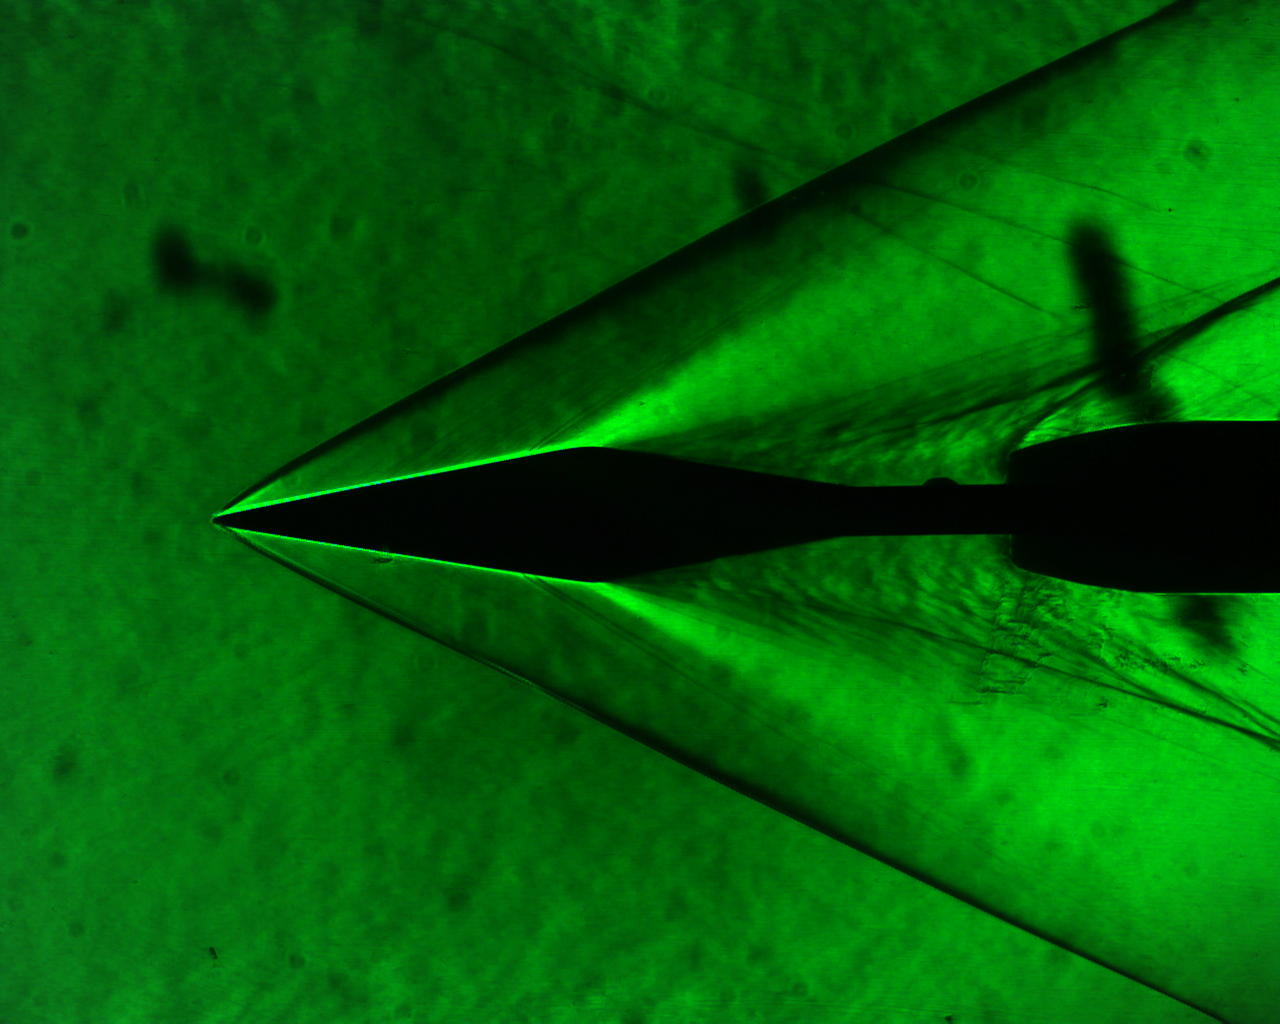
\includegraphics[width = \linewidth]{images/diamond_vertical_AoA0_M3.png}  
    \caption{ASE 162M High-Speed Aerodynamics}
  \end{subfigure} 
  \vspace{4mm}

  \begin{subfigure}{0.75\linewidth}
    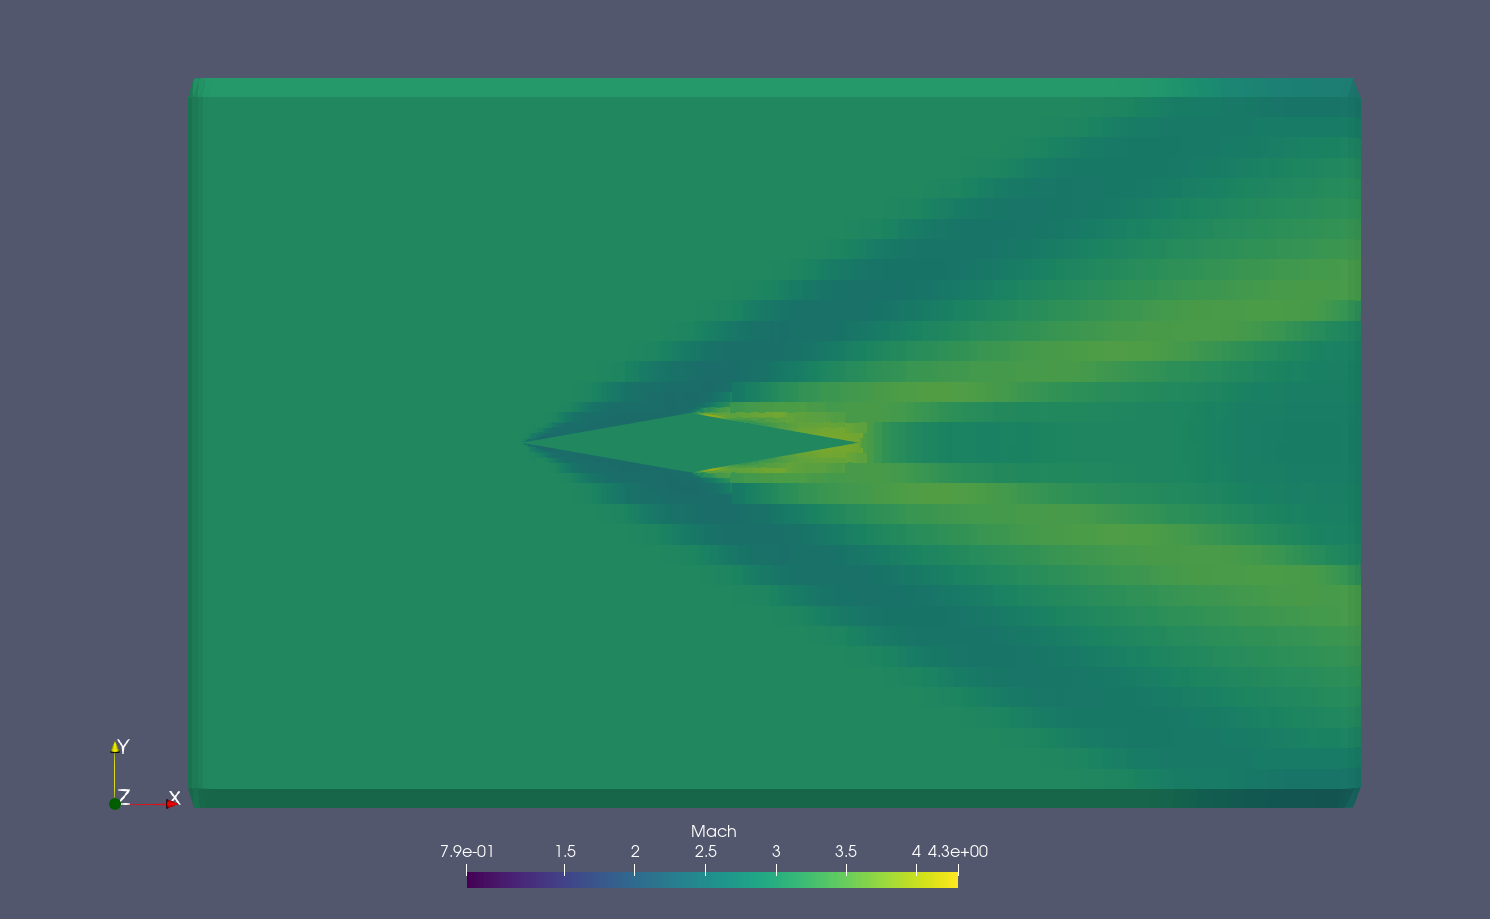
\includegraphics[width = \linewidth]{images/3D_Diamond_Sim_Coarse_Mach_PARAVIEW.png}  
    \caption{Slice of the 3D Result showing Mach No.}
  \end{subfigure} 

  \caption{Comparison between the simulation and a real wind tunnel at Mach 3}
  \label{3dshi}
\end{figure}

A previous experiment involving a schlieren step for visualization of supersonic flow in \textit{High Speed Aerodynamics, ASE 162M} shows flow with a freestream Mach number \(M_\infty = 3\) over the diamond airfoil at \(\alpha=0^\circ\), the experimentally measured shock‐wave angle was
\[
\beta_{\rm exp} = 28.73^\circ,
\]
while our 3D CFD simulation yielded
\[
\beta_{\rm sim} = 30.54^\circ,
\]
an overprediction of \(\Delta\beta = +1.81^\circ\) (\(\approx6.3\%\)). 

The discrepancy likely arises from three‐dimensional flow expansion and residual numerical diffusion in the shock region.  Despite the overestimate, the mesh resolution captures the overall 3D shock structure well, and further local refinement or higher‐order schemes could reduce the remaining error. 

However, $\beta_{3D} \approx 30.54 \degree$, which is greater than the theoretical result from 2D Euler Equations, $\beta_{\rm theory}=27.38^\circ$. Due to 3D effects, the wave angle is expected to be greater given the flow relief in the spanwise direction. This turns out to be the case for this mesh.
\vspace{1.5mm}

The shocks and expansion fans are not as clear as they were in the 2D simulations. It appears transparent like vapour, which is a key visual aspect of a real supersonic shock!
\vspace{1.5mm}

Stats on this "coarse" mesh : $N_{cells} = 947084$, $N_{faces} = 3072728$, and $N_{points} = 1178825$.


\section{Conclusion}

A systematic mesh‐refinement study in two dimensions demonstrated that the computed oblique‐shock angle converges to within $0.1^\circ$ of the theoretical value $\beta_{\rm theory}=27.38^\circ$, and the apex stagnation pressure agrees within 1 percent of theory—validating the mesh and solver fidelity for 2D inviscid flow.

When extended to a structured 3D mesh ($\approx \times 10^6$ cells), the predicted wave angle increases to
\[
  \beta_{\rm sim,3D} = 30.54^\circ,
\]
moving the solution toward the experimental measurement $\beta_{\rm exp}=28.73^\circ$ and correctly capturing the characteristic steepening due to spanwise flow relief and boundary‐layer effects. Although the absolute error relative to experiment is $+1.81^\circ$ (6.3\%), the 3D simulation reproduces the observed trend that 2D Euler theory cannot.

In summary, while 2D inviscid theory and simulation agree with high precision, the 3D CFD model more faithfully reproduces experimental shock‐wave behavior in finite‐span diamond airfoils, underscoring the importance of three‐dimensional effects in supersonic aerodynamics.


\pagebreak
\appendix
\pagenumbering{gobble} 
\begin{center}
\vspace*{\fill}
   \Huge \bf Appendix 
\vspace*{\fill}
\end{center}
\pagebreak 

\hypertarget{code}{}
\section{Code}
% PDF of code starts on next page. 
% \vspace{2.5mm}

Additionally, team repository: \url{https://github.com/andressuniaga/CFD-SP25-11}
\vspace{2.5mm}

\end{document}